% ============================================================
%  INFORME FINAL — PRÁCTICA EXPERIMENTAL UNIDAD III
%  SGED: Sistema de Gestión para Escuela Deportiva ProFútbol
%  Universidad Técnica Estatal de Quevedo
% ============================================================
\documentclass[12pt]{article}
\usepackage[spanish]{babel}
\usepackage[utf8]{inputenc}
\usepackage[T1]{fontenc}
\usepackage{graphicx}
\usepackage{geometry}
\usepackage{setspace}
\usepackage[hidelinks]{hyperref}
\usepackage{float}
\usepackage{titlesec}
\usepackage{listings}
\usepackage{xcolor}
\usepackage{enumitem}
\usepackage{amsmath}
\usepackage{booktabs}
\usepackage{array}
\usepackage{longtable}
\usepackage{fancyhdr}
\usepackage{tocloft}
\usepackage{mdframed}

\geometry{a4paper, margin=2.5cm}
\setstretch{1.15}

% --- Rutas de imágenes ---
\graphicspath{{evidencias/}{arquitectura/}}

% --- Configuración para código ---
\definecolor{codegreen}{rgb}{0,0.6,0}
\definecolor{codegray}{rgb}{0.5,0.5,0.5}
\definecolor{backcolour}{rgb}{0.95,0.95,0.92}

\lstset{
	backgroundcolor=\color{backcolour},
	commentstyle=\color{codegreen},
	keywordstyle=\color{blue},
	numberstyle=\tiny\color{codegray},
	stringstyle=\color{orange},
	basicstyle=\ttfamily\footnotesize,
	breaklines=true,
	captionpos=b,
	numbers=left,
}

% --- Entorno para box de pendiente ---
\newmdenv[
linecolor=orange!70,
backgroundcolor=orange!8,
linewidth=1.5pt,
roundcorner=4pt,
frametitle={\color{orange!80!black}\bfseries PENDIENTE — ALEJANDRO (Paso 5: Network Tab)},
frametitlealignment=\centering
]{pendientebox}

% --- Encabezado / pie de página ---
\pagestyle{fancy}
\fancyhf{}
\fancyhead[L]{\small SGED — Práctica Experimental U3}
\fancyhead[R]{\small UTEQ — Aplicaciones Web}
\fancyfoot[C]{\thepage}
\renewcommand{\headrulewidth}{0.4pt}

% ============================================================
\begin{document}
	
	% ============================================================
	%  PORTADA
	% ============================================================
	\begin{titlepage}
		\begin{center}
			\includegraphics[width=0.22\textwidth]{logo-uteq.png} \\[0.4cm]
			{\large \textbf{UNIVERSIDAD TÉCNICA ESTATAL DE QUEVEDO}} \\[0.2cm]
			{\large \textbf{FACULTAD DE CIENCIAS DE LA COMPUTACIÓN Y DISEÑO DIGITAL}} \\[0.2cm]
			{\large \textbf{CARRERA DE INGENIERÍA EN SOFTWARE}} \\[0.2cm]
			
			\rule{\linewidth}{0.5pt} \\[0.1cm]
			{\Large \textbf{INFORME DE PRÁCTICA EXPERIMENTAL}} \\[0.2cm]
			{\large \textbf{UNIDAD III}} \\[0.2cm]
			\rule{\linewidth}{0.5pt} \\[0.1cm]
			
			\textbf{TEMA:} \\[0.2cm]
			{\Large \textbf{Sistema de Gestión para la Escuela Deportiva ProFútbol}} \\[0.2cm]
			{\large Arquitectura Monolítica por Capas con Spring Boot, Angular y PostgreSQL\\
				Implementación de ORM, Caché Redis, JWT y Patrones de Arquitectura} \\[0.5cm]
			
			\textbf{INTEGRANTES:} \\[0.2cm]
			\begin{tabular}{l}
				\textbf{BELTRÁN MONTIEL FRED ADRIÁN} \\[0.2cm]
				\textbf{CRUZ PÉREZ JUSTYN KEITH} \\[0.2cm]
				\textbf{PALLO PINTO DANIEL ALEJANDRO} \\[0.2cm]
			\end{tabular} \\[0.2cm]
			
			\textbf{DOCENTE:} \\[0.2cm]
			ING. GUERRERO ULLOA GLEISTON CICERÓN \\[0.2cm]
			
			\textbf{MATERIA:} \\[0.2cm]
			APLICACIONES WEB — A — [5to Nivel] \\[0.2cm]
			
			\textbf{REPOSITORIO DE GITHUB:}\\[0.2cm]
			\url{https://github.com/Alejandro-hub19/SGED_Practicas_U3}\\[0.5cm]
			
			\vfill
			\rule{0.5\linewidth}{0.4pt} \\[0.1cm]
			Quevedo — Ecuador \\
			2026
		\end{center}
	\end{titlepage}
	
	\newpage
	
	% ============================================================
	%  TABLA DE CONTENIDOS
	% ============================================================
	\tableofcontents
	\newpage
	
	% ============================================================
	%  SECCIÓN 1 — DESCRIPCIÓN DE LA PRÁCTICA
	% ============================================================
	\section{Descripción de la Práctica}
	
	La presente práctica de laboratorio de la Unidad III corresponde al desarrollo del \textbf{Sistema de Gestión para la Escuela Deportiva ProFútbol (SGED)}, una aplicación web de gestión administrativa y deportiva implementada de forma progresiva a lo largo del ciclo académico.
	
	El sistema centraliza la administración de estudiantes, entrenadores, asistencias, membresías y evaluaciones de rendimiento en una plataforma única, construida sobre un stack tecnológico moderno:
	
	\begin{itemize}
		\item \textbf{Backend:} Java 21 con Spring Boot 3.x (REST API, Spring Data JPA, Spring Security, Flyway)
		\item \textbf{Frontend:} Angular 17+ (SPA, Angular Router, HttpClient con interceptores JWT)
		\item \textbf{Base de Datos:} PostgreSQL con migraciones gestionadas por Flyway
		\item \textbf{Caché:} Redis (patrón Cache-Aside + Blacklist de tokens JWT)
		\item \textbf{Testing:} JUnit 5, Mockito, JaCoCo (cobertura del 96\%)
		\item \textbf{Infraestructura local:} Docker Compose
	\end{itemize}
	
	La arquitectura adoptada es un \textbf{Monolito por Capas} (Presentación $\rightarrow$ Controladores $\rightarrow$ Servicios $\rightarrow$ Acceso a Datos), decisión documentada y justified en los Architecture Decision Records (ADRs) incluidos en este informe.
	
	La práctica evidencia el flujo completo de integración: desde las migraciones de esquema con Flyway, hasta la exposición de endpoints REST consumidos por Angular, pasando por la capa de caché con Redis y los mecanismos de autenticación JWT con invalidación en tiempo real.
	
	\newpage
	
	% ============================================================
	%  SECCIÓN 2 — FUNDAMENTO TEÓRICO
	% ============================================================
	\section{Fundamento Teórico}
	
	% -----------------------------------------------------------
	\subsection{5.2 ORM y Mapeo Objeto-Relacional}
	\textit{(Elaborado por: Cruz Pérez Justyn Keith)}
	
	El uso de un Mapeo Objeto-Relacional (ORM) surge como solución a una de las dificultades más prominentes en la ingeniería de software: el \textit{Object-Relational Impedance Mismatch} (desajuste de impedancia objeto-relacional). Este problema se origina porque los paradigmas orientados a objetos y los relacionales están fundamentados en principios teóricos distintos. Mientras que la orientación a objetos se basa en la encapsulación, herencia, polimorfismo y la identidad en memoria, las bases de datos relacionales operan bajo la teoría matemática de conjuntos y el álgebra relacional, utilizando tablas, filas y claves foráneas (Ambler, 2003). Esto genera conflictos en la representación de datos, tales como la granularidad (objetos complejos frente a tablas planas), la direccionalidad de las asociaciones y, fundamentalmente, la herencia, la cual no existe nativamente en SQL estándar.
	
	Para solventar la carencia de herencia relacional, los ORM proveen tres estrategias principales de mapeo (Fowler, 2002):
	
	\begin{enumerate}
		\item \textbf{Single Table (Tabla Única):} Mapea toda la jerarquía de clases a una sola tabla, empleando una columna ``discriminadora'' para identificar a qué subclase pertenece cada fila. Es ideal para jerarquías simples donde las subclases añaden pocos atributos específicos. Su ventaja es el alto rendimiento (no requiere \textit{JOINs}), pero genera tablas dispersas con valores nulos e impide usar restricciones \texttt{NOT NULL} en columnas de las subclases.
		
		\item \textbf{Class Table o Joined (Tabla por Clase):} Cada clase de la jerarquía tiene su propia tabla. Las tablas de las subclases contienen solo sus campos específicos y una clave foránea hacia la tabla de la superclase. Recomendada para jerarquías complejas y profundas, aunque consultar datos de una subclase requiere múltiples operaciones \textit{JOIN}.
		
		\item \textbf{Concrete Table (Tabla por Clase Concreta):} Cada clase instanciable posee su propia tabla con todos sus atributos (incluidos los heredados). Útil cuando rara vez se realizan consultas polimórficas, pero la desventaja es que alterar un atributo en la superclase obliga a modificar el esquema de múltiples tablas.
	\end{enumerate}
	
	\subsubsection*{Tabla Comparativa: ORM vs.\ SQL Puro vs.\ Query Builder}
	
	\begin{table}[H]
		\centering
		\resizebox{\textwidth}{!}{%
			\begin{tabular}{@{}p{3.2cm}p{4.5cm}p{4.5cm}p{4.5cm}@{}}
				\toprule
				\textbf{Criterio} & \textbf{ORM (Hibernate/JPA)} & \textbf{SQL Puro (JDBC)} & \textbf{Query Builder (jOOQ)} \\ \midrule
				\textbf{Curva de aprendizaje} & Alta (ciclo de vida, lazy loading, caché). & Baja–Media (requiere dominio de SQL). & Media (API específica de la herramienta). \\[4pt]
				\textbf{Rendimiento simple} & Bueno (overhead mitigado por caché). & Excelente (sin abstracciones). & Muy Bueno (traducción directa a SQL). \\[4pt]
				\textbf{Problema N+1} & Riesgo alto si no se configuran fetch types. & Sin riesgo inherente. & Sin riesgo; genera el JOIN explícito. \\[4pt]
				\textbf{Portabilidad} & Alta (dialecto del ORM). & Baja (SQL dependiente del motor). & Media/Alta. \\[4pt]
				\textbf{Migraciones} & Media (generación automática con ajustes). & N/A (requiere Flyway externo). & N/A (complemento externo). \\[4pt]
				\textbf{Debugging} & Difícil (SQL generado oscuro). & Fácil (query explícito). & Fácil (código Java similar al query). \\
				\bottomrule
			\end{tabular}%
		}
		\caption{Comparativa de tecnologías de acceso a datos.}
	\end{table}
	
	% -----------------------------------------------------------
	\subsection{5.3 Patrones de Arquitectura para Aplicaciones Web Escalables}
	\textit{(Elaborado por: Cruz Pérez Justyn Keith)}
	
	En el desarrollo de aplicaciones web a escala, el éxito no solo depende del código implementado, sino de cómo se toman, comunican y preservan las decisiones de diseño. Según la Guía del Cuerpo de Conocimiento de Ingeniería de Software (SWEBOK v4.0), la ingeniería de software se distingue de la simple programación por su énfasis en la documentación del diseño y el razonamiento arquitectónico (Bourque \& Fairley, 2014).
	
	Para institucionalizar el registro de decisiones, Michael Nygard propuso el formato de \textbf{Architecture Decision Records (ADR)} (Nygard, 2011). Un ADR es un documento corto almacenado junto al código fuente que captura una decisión arquitectónica importante. El formato estándar se compone de:
	
	\begin{enumerate}
		\item \textbf{Título:} Identificador corto y descriptivo (ej.\ ``ADR-003: Uso de Redis para Caché'').
		\item \textbf{Estado:} Indica si está propuesto, aceptado, rechazado o deprecado.
		\item \textbf{Contexto:} Describe las fuerzas en juego, el problema a resolver y los limitantes tecnológicos.
		\item \textbf{Decisión:} La elección tomada formulada de manera asertiva y clara.
		\item \textbf{Consecuencias:} Describe el resultado final, tanto positivo como negativo (\textit{trade-offs}).
	\end{enumerate}
	
	Al seguir el estándar de Nygard, los equipos aseguran que la evolución del sistema sea trazable y que las decisiones se justifiquen en el momento histórico de su adopción, un principio cardinal de la ingeniería de software madura.
	
	\subsubsection*{Análisis de Escalabilidad del Monolito SGED}
	
	Nuestro ADR-001 establece la utilización de una \textbf{Arquitectura Monolítica por Capas} para el proyecto SGED. Al contrastar esto con la literatura, el caso de \textbf{Shopify} ilustra que un monolito bien estructurado puede operar exitosamente a escala global antes de contemplar siquiera la separación física de componentes (Deobald, 2018). La literatura respalda que un monolito bien estructurado supera a un sistema de microservicios prematuro que introduce latencia de red y complejidad operativa (Fowler, \textit{Microservice Premium}).
	
	Sin embargo, si el SGED debiera escalar masivamente, los siguientes módulos representarían cuellos de botella:
	
	\begin{itemize}
		\item \textbf{Módulo de Evaluaciones y Asistencias:} Durante cierres de ciclo, el ingreso masivo generaría picos de transacciones. Se beneficiaría de una arquitectura orientada a eventos (EDA) o un microservicio independiente.
		\item \textbf{Gestión de Notificaciones:} Procesarlo dentro del hilo monolítico bloquearía la aplicación; requeriría una arquitectura orientada a colas (RabbitMQ/Kafka).
		\item \textbf{Base de Datos Única (PostgreSQL):} Con el escalamiento horizontal, requeriría réplicas de lectura (\textit{Read Replicas}) o \textit{Sharding}, complementado con el Cache-Aside ya implementado con Redis.
	\end{itemize}
	
	% -----------------------------------------------------------
	\subsection{5.4 Caché: Patrones y Medición de Rendimiento}
	\textit{(Elaborado por: Beltrán Montiel Fred Adrián)}
	
	Una aplicación web moderna puede cachear datos en varios niveles, cada uno con su propio TTL y estrategia de invalidación. En el \textbf{navegador}, las cabeceras \texttt{Cache-Control} y \texttt{ETag} permiten que el cliente reutilice respuestas sin volver a pedirlas al servidor. Un \textbf{CDN} cachea contenido estático cerca geográficamente del usuario. A nivel de \textbf{base de datos}, Redis actúa como capa intermedia entre la aplicación y PostgreSQL, con TTLs cortos (minutos) e invalidación activa mediante \texttt{@CacheEvict}.
	
	\subsubsection*{Patrones de Caché}
	
	\begin{itemize}
		\item \textbf{Cache-Aside} (el implementado en este proyecto): la aplicación consulta primero Redis; si hay \textit{hit}, devuelve el valor sin tocar la base de datos; si hay \textit{miss}, consulta PostgreSQL, guarda el resultado en Redis y lo devuelve. \\
		Secuencia: \texttt{Cliente $\rightarrow$ Service $\rightarrow$ Redis (miss) $\rightarrow$ Repository $\rightarrow$ PostgreSQL $\rightarrow$ Redis (guardar) $\rightarrow$ Cliente}
		
		\item \textbf{Read-Through:} la aplicación nunca habla directamente con la base; siempre pasa por una capa de caché que internamente decide si consulta la fuente. La diferencia con Cache-Aside es que la lógica de ``ir a buscar a la base'' vive en la capa de caché, no en el Service.
		
		\item \textbf{Write-Through:} cada escritura se guarda simultáneamente en caché y en base de datos, de forma síncrona. Garantiza consistencia inmediata, pero añade latencia a cada escritura.
		
		\item \textbf{Write-Behind} (\textit{write-back}): la escritura se guarda primero en caché y se persiste a la base de datos de forma asíncrona, en lotes o tras un \textit{delay}. Mejora el rendimiento de escritura, pero arriesga pérdida de datos si Redis falla antes de persistir.
	\end{itemize}
	
	\subsubsection*{Cache Stampede y su Mitigación}
	
	El \textit{cache stampede} ocurre cuando una clave popular expira y, en el mismo instante, múltiples peticiones concurrentes detectan el \textit{miss} y golpean todas a la base de datos a la vez, anulando el beneficio de la caché. Se mitiga con:
	
	\begin{enumerate}
		\item Un \textbf{mutex/lock} que permite que solo una petición regenere el valor mientras las demás esperan.
		\item \textbf{Expiración probabilística temprana} (\textit{probabilistic early expiration}), donde se recalcula el valor un poco antes de que expire realmente, distribuyendo la carga de regeneración en el tiempo.
	\end{enumerate}
	
	\subsubsection*{Estructuras de Datos de Redis en el Proyecto}
	
	Redis no es solo un almacén clave-valor simple; ofrece varias estructuras, de las cuales el proyecto utiliza:
	
	\begin{itemize}
		\item \textbf{Strings:} usada para guardar el JSON serializado del \texttt{PageResponse} (cache-aside de estudiantes, vía \texttt{RedisCacheManager}).
		\item \textbf{Keys con TTL individual:} para la blacklist de JWT —cada token revocado se almacena con un TTL igual a la vida restante del token original, garantizando que Redis se limpie automáticamente sin crecimiento infinito de memoria.
	\end{itemize}
	
	\subsubsection*{Metodología de Benchmarking}
	
	Para medir el impacto real de la caché se aplica la siguiente metodología:
	
	\begin{enumerate}
		\item Tamaño de muestra $n \geq 10$ corridas por escenario para evitar que un dato atípico distorsione la conclusión.
		\item Reportar \textbf{media y desviación estándar}, no solo el promedio, ya que una alta dispersión indica inconsistencia.
		\item \textbf{Aislar la variable}: correr exactamente la misma consulta con los mismos datos, cambiando únicamente si la caché está activa (\texttt{SPRING\_CACHE\_TYPE=redis}) o no (\texttt{none}).
	\end{enumerate}
	
	El resultado se expresa como \textit{speedup}: $S = T_{\text{sin}} / T_{\text{con}}$, donde $S > 1$ indica mejora y $S > 2$ es el umbral que justifica la complejidad operacional añadida. Los resultados obtenidos muestran un speedup de \textbf{2.07x} (media) y \textbf{2.24x} (percentil 95), superando el umbral establecido.
	
	\newpage
	
	% ============================================================
	%  SECCIÓN 3 — ARQUITECTURA DEL SISTEMA
	% ============================================================
	\section{Arquitectura del Sistema}
	
	\subsection{Diagrama C4 — Nivel 1: Contexto}
	
	\begin{figure}[H]
		\centering
		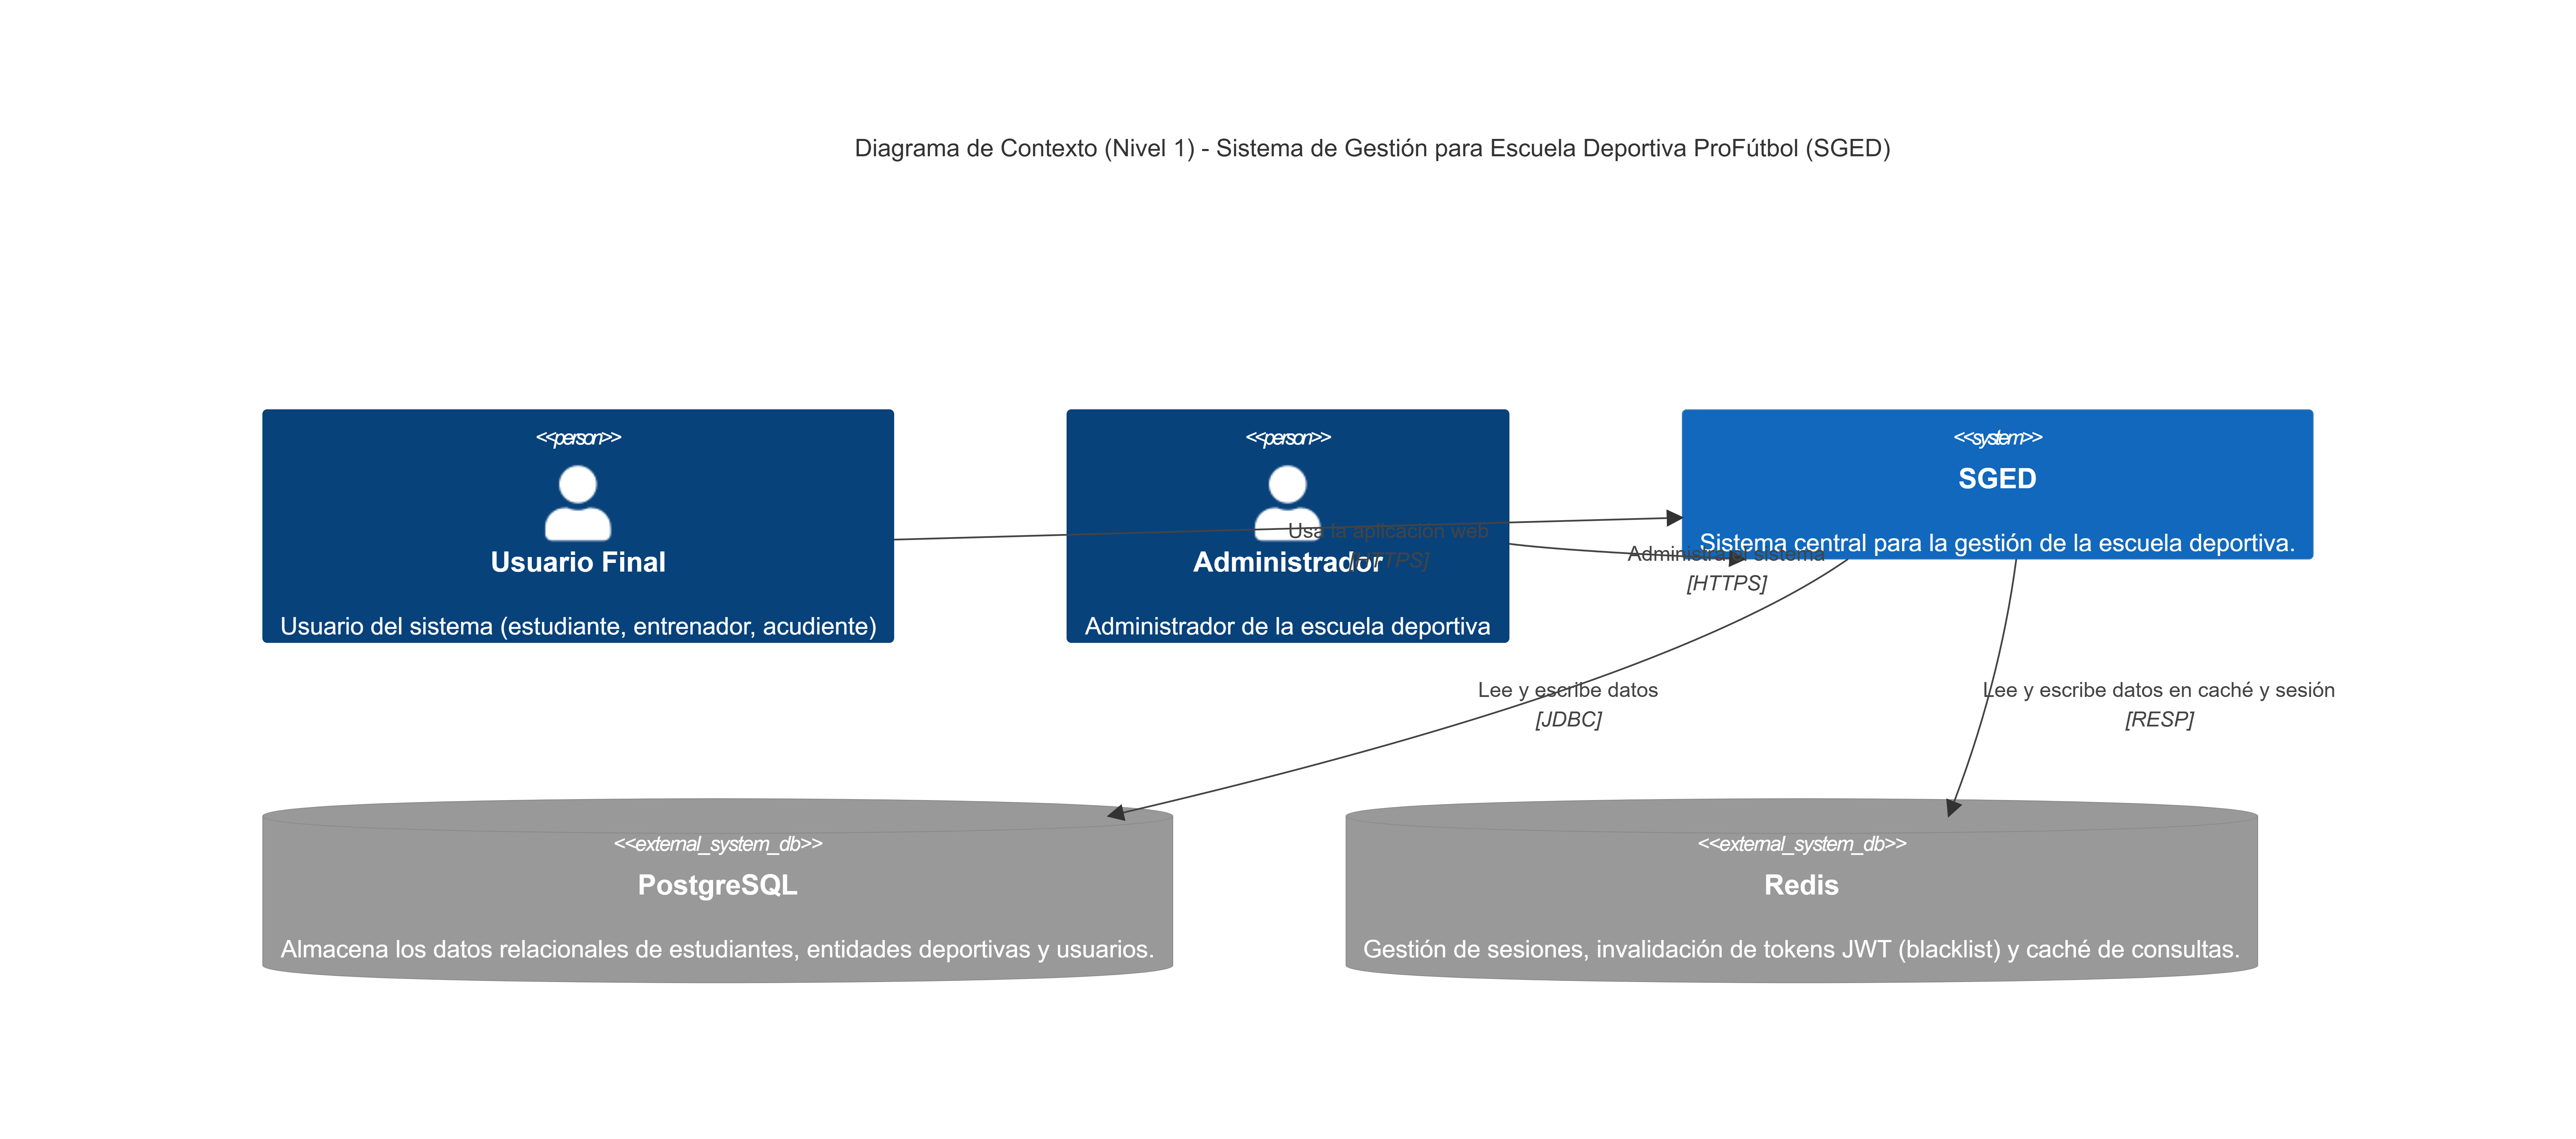
\includegraphics[width=0.85\textwidth]{C4_1_Contexto.png}
		\caption{Diagrama C4 Nivel 1 — Contexto del sistema SGED.}
	\end{figure}
	
	\subsection{Diagrama C4 — Nivel 2: Contenedores}
	
	\begin{figure}[H]
		\centering
		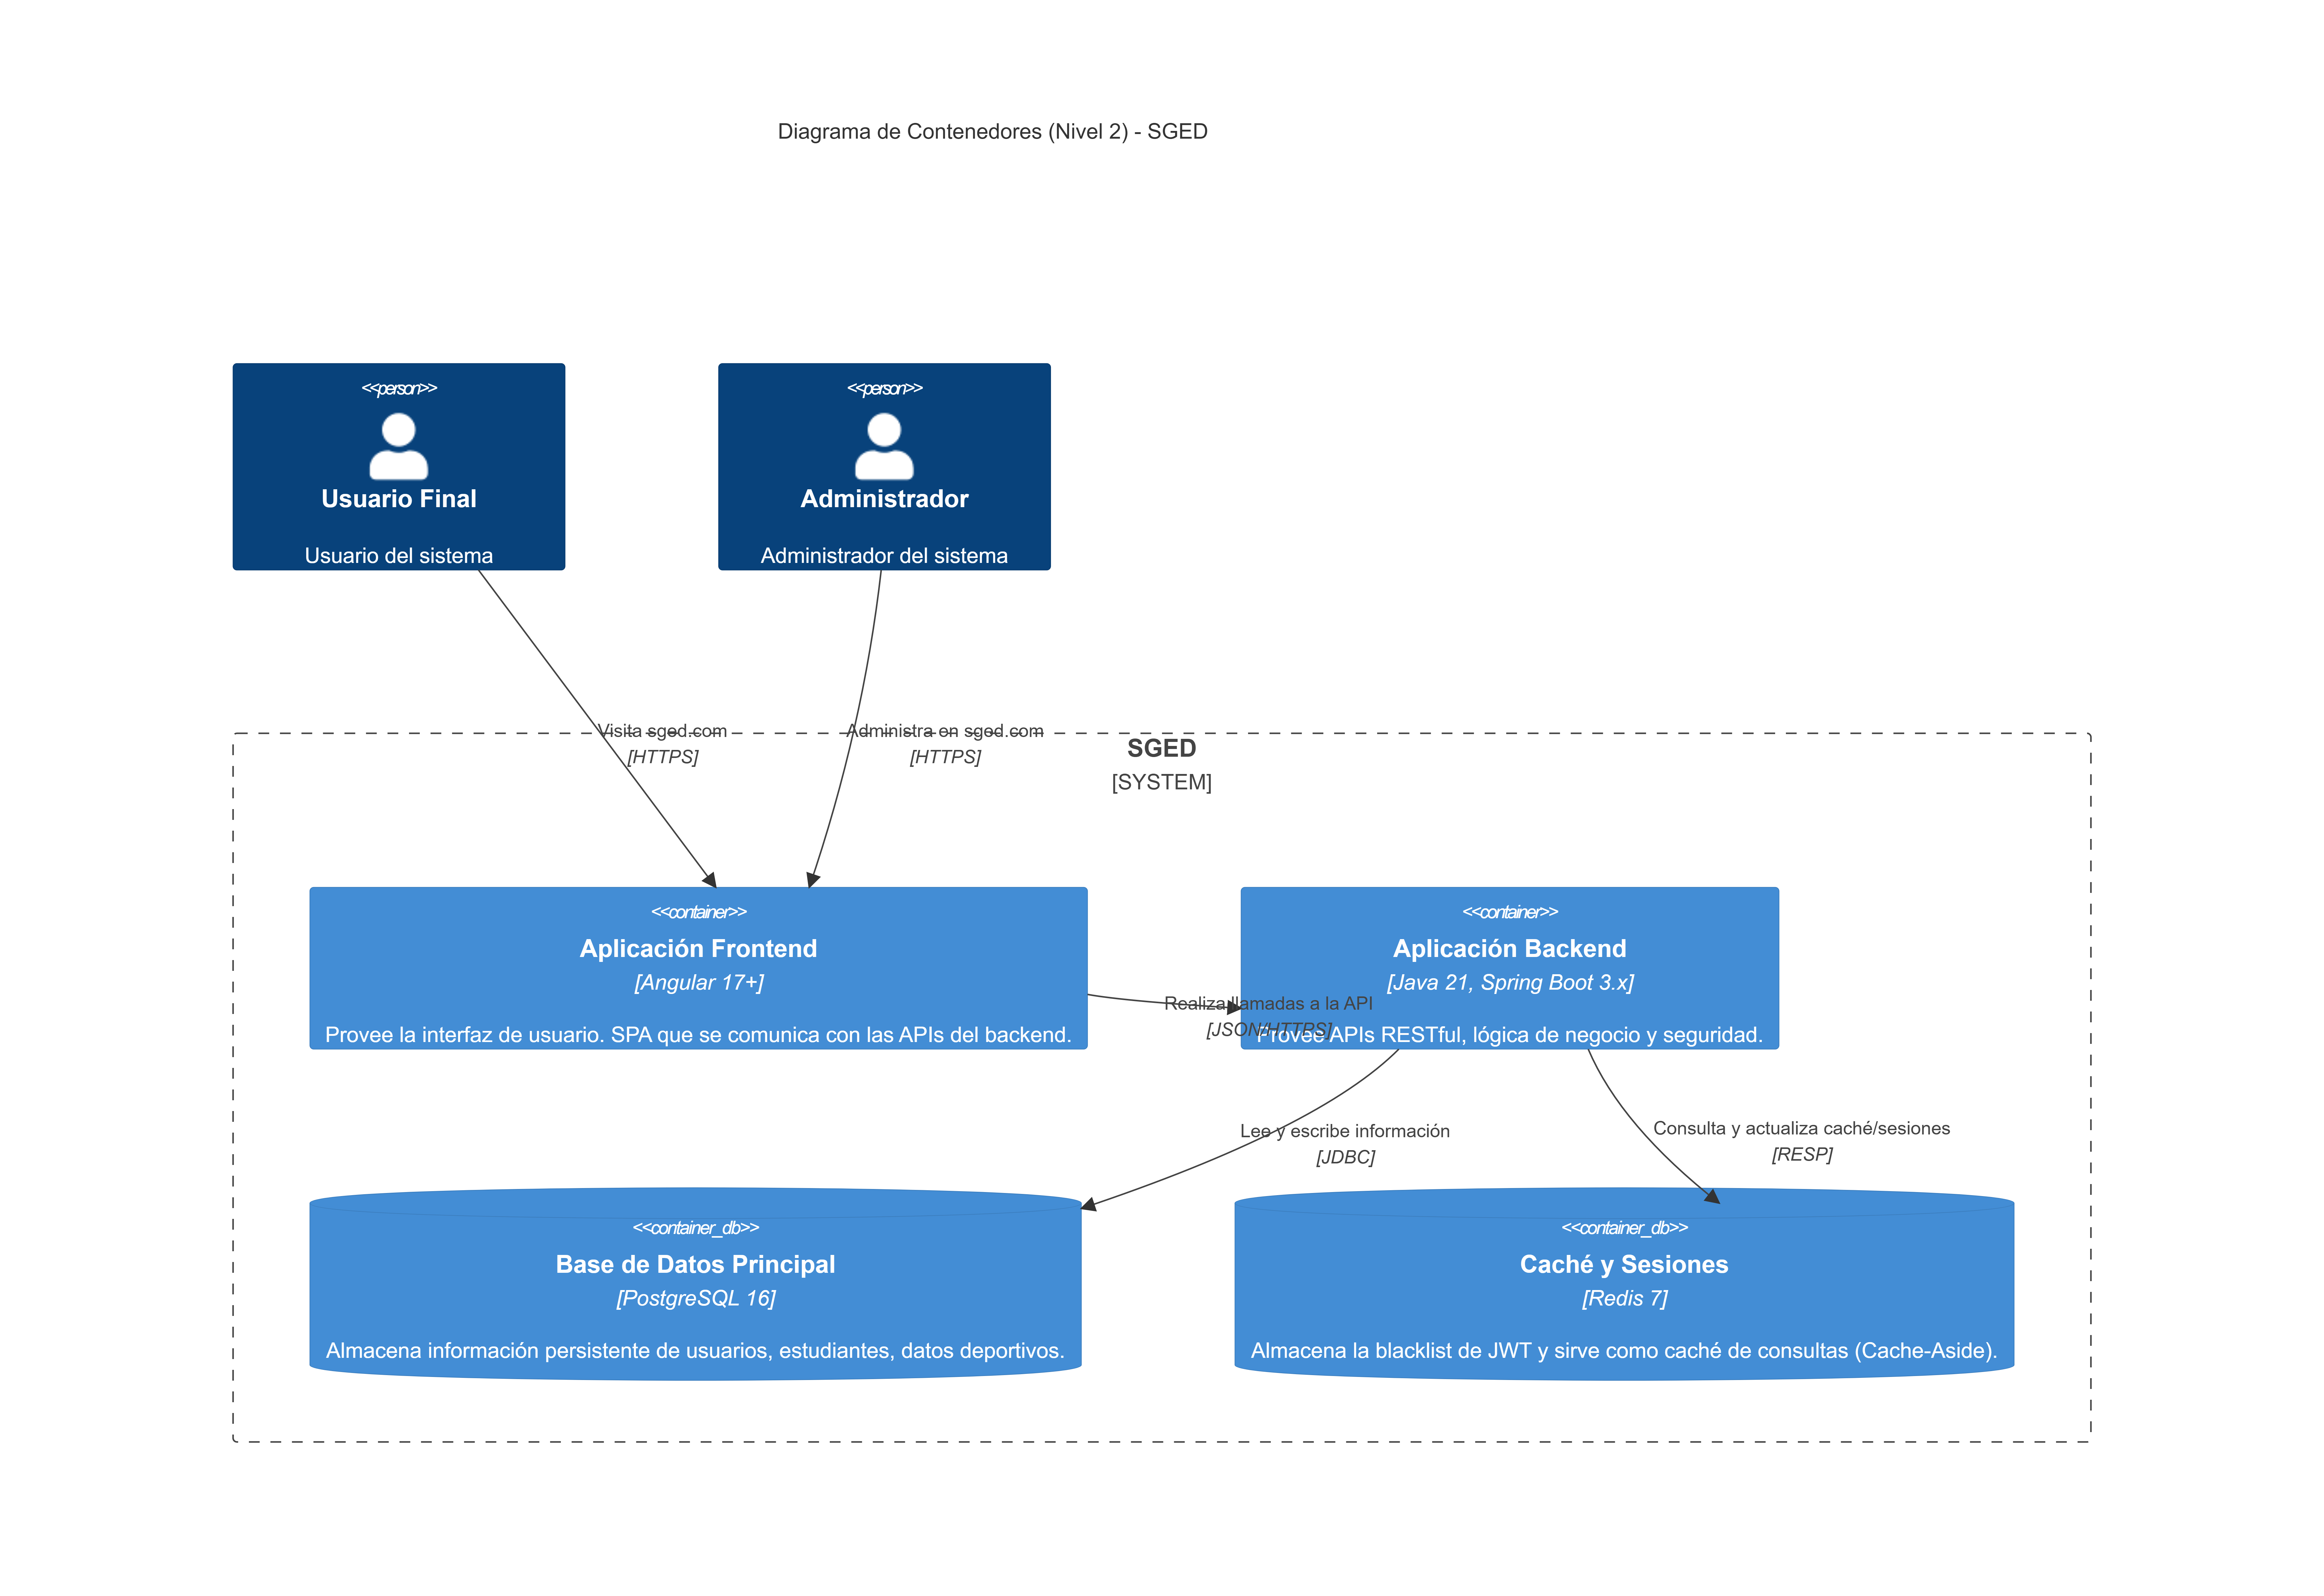
\includegraphics[width=0.88\textwidth]{C4_2_Contenedores.png}
		\caption{Diagrama C4 Nivel 2 — Contenedores: Angular, Spring Boot, PostgreSQL y Redis.}
	\end{figure}
	
	\subsection{Diagrama C4 — Nivel 3: Componentes}
	
	\begin{figure}[H]
		\centering
		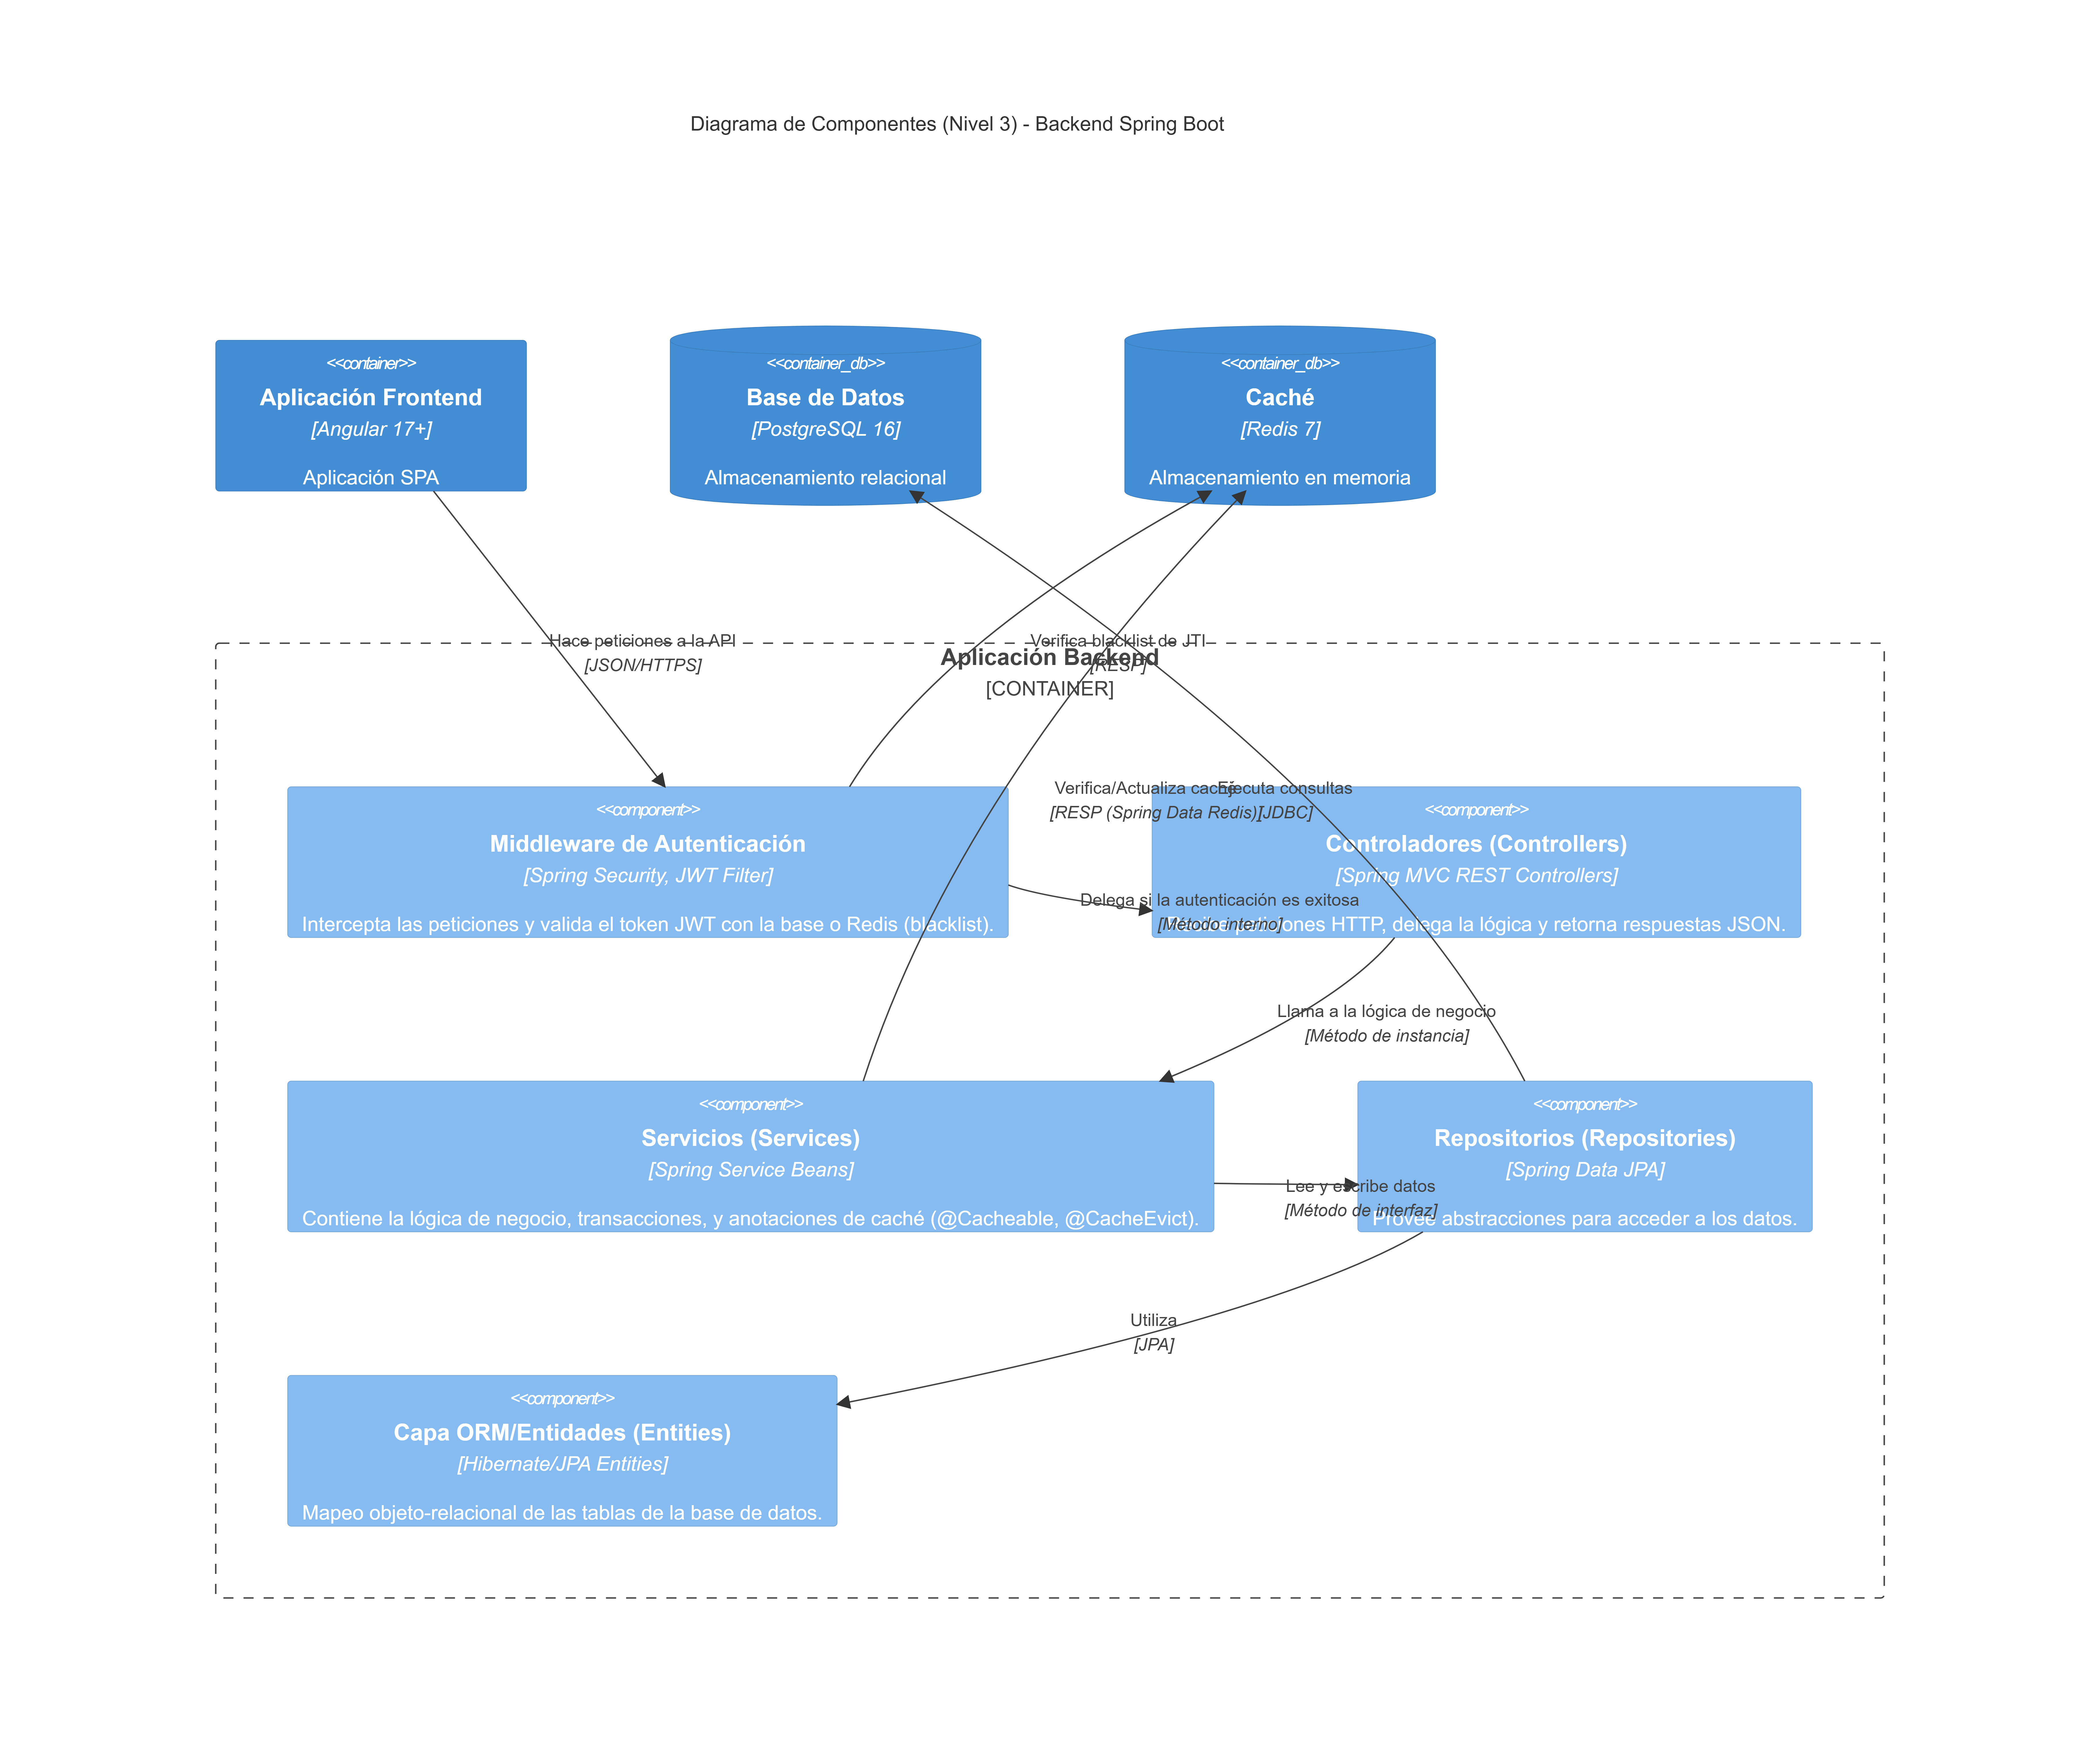
\includegraphics[width=0.88\textwidth]{C4_3_Componentes.png}
		\caption{Diagrama C4 Nivel 3 — Componentes internos del backend Spring Boot.}
	\end{figure}
	
	\subsection{Diagrama de Clases}
	
	\begin{figure}[H]
		\centering
		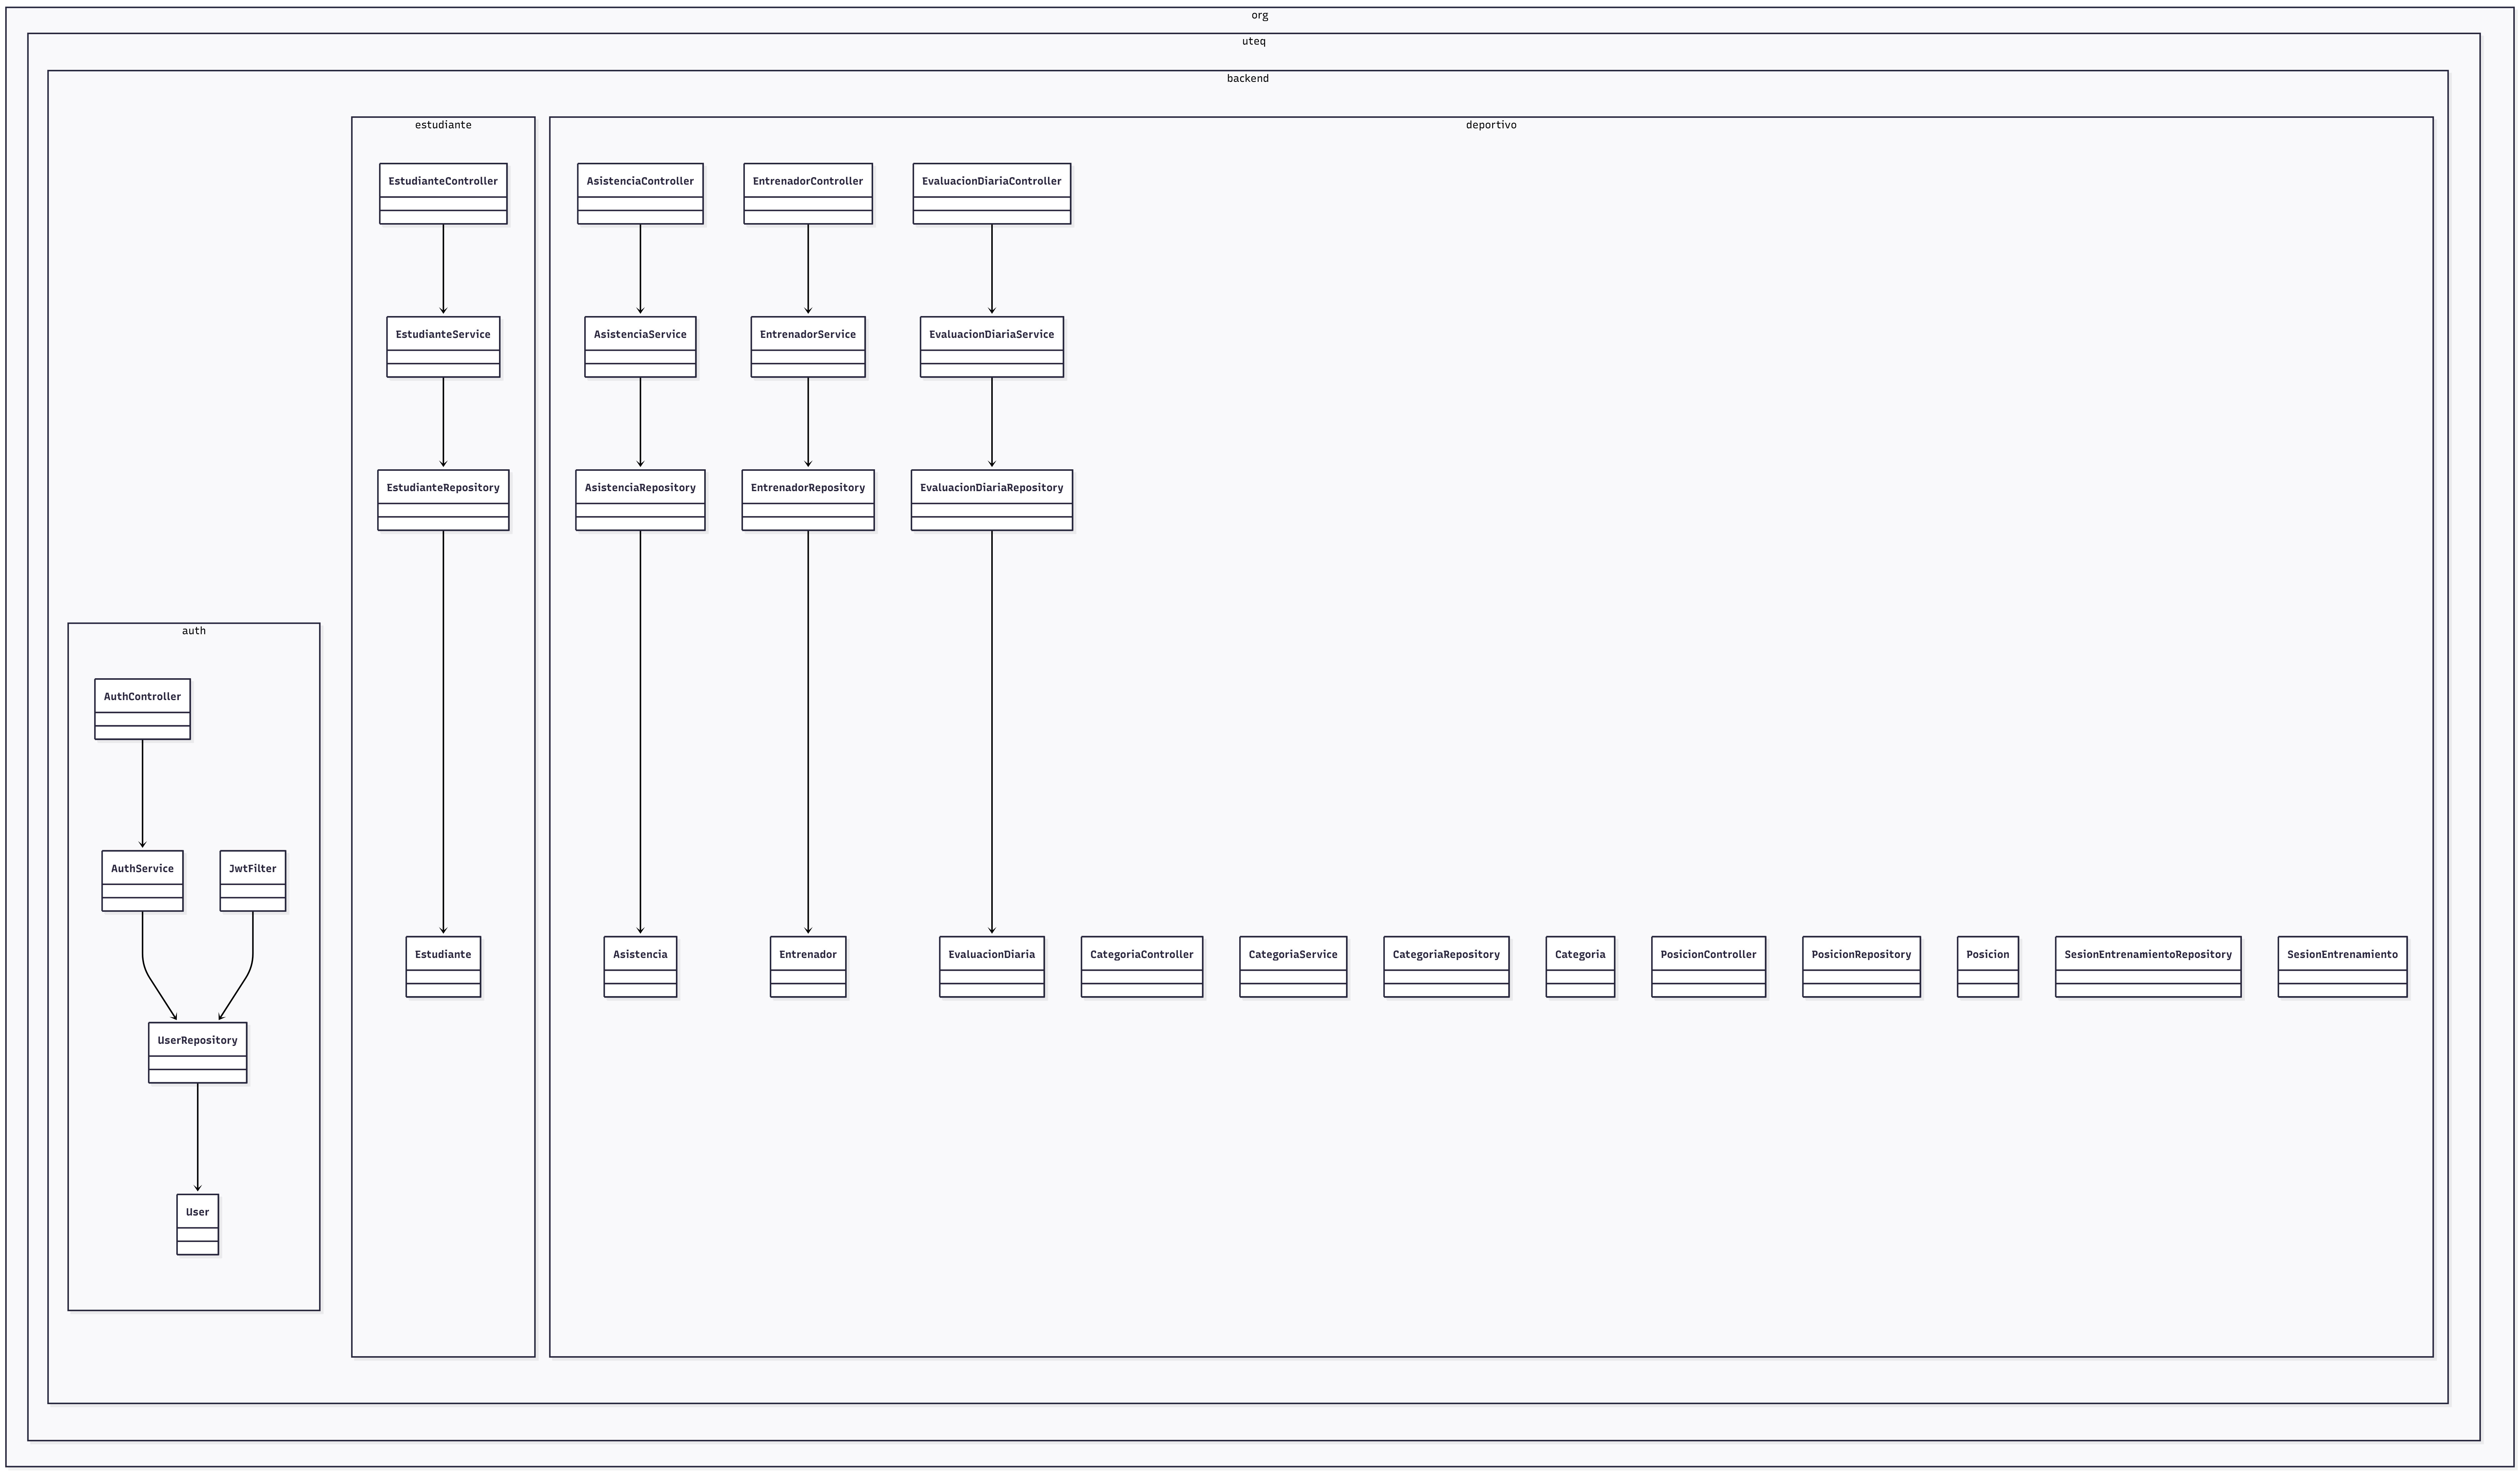
\includegraphics[width=0.88\textwidth]{Diagrama_Clases.png}
		\caption{Diagrama de Clases del dominio SGED.}
	\end{figure}
	
	\subsection{Diagrama ERD — Modelo Relacional}
	
	\begin{figure}[H]
		\centering
		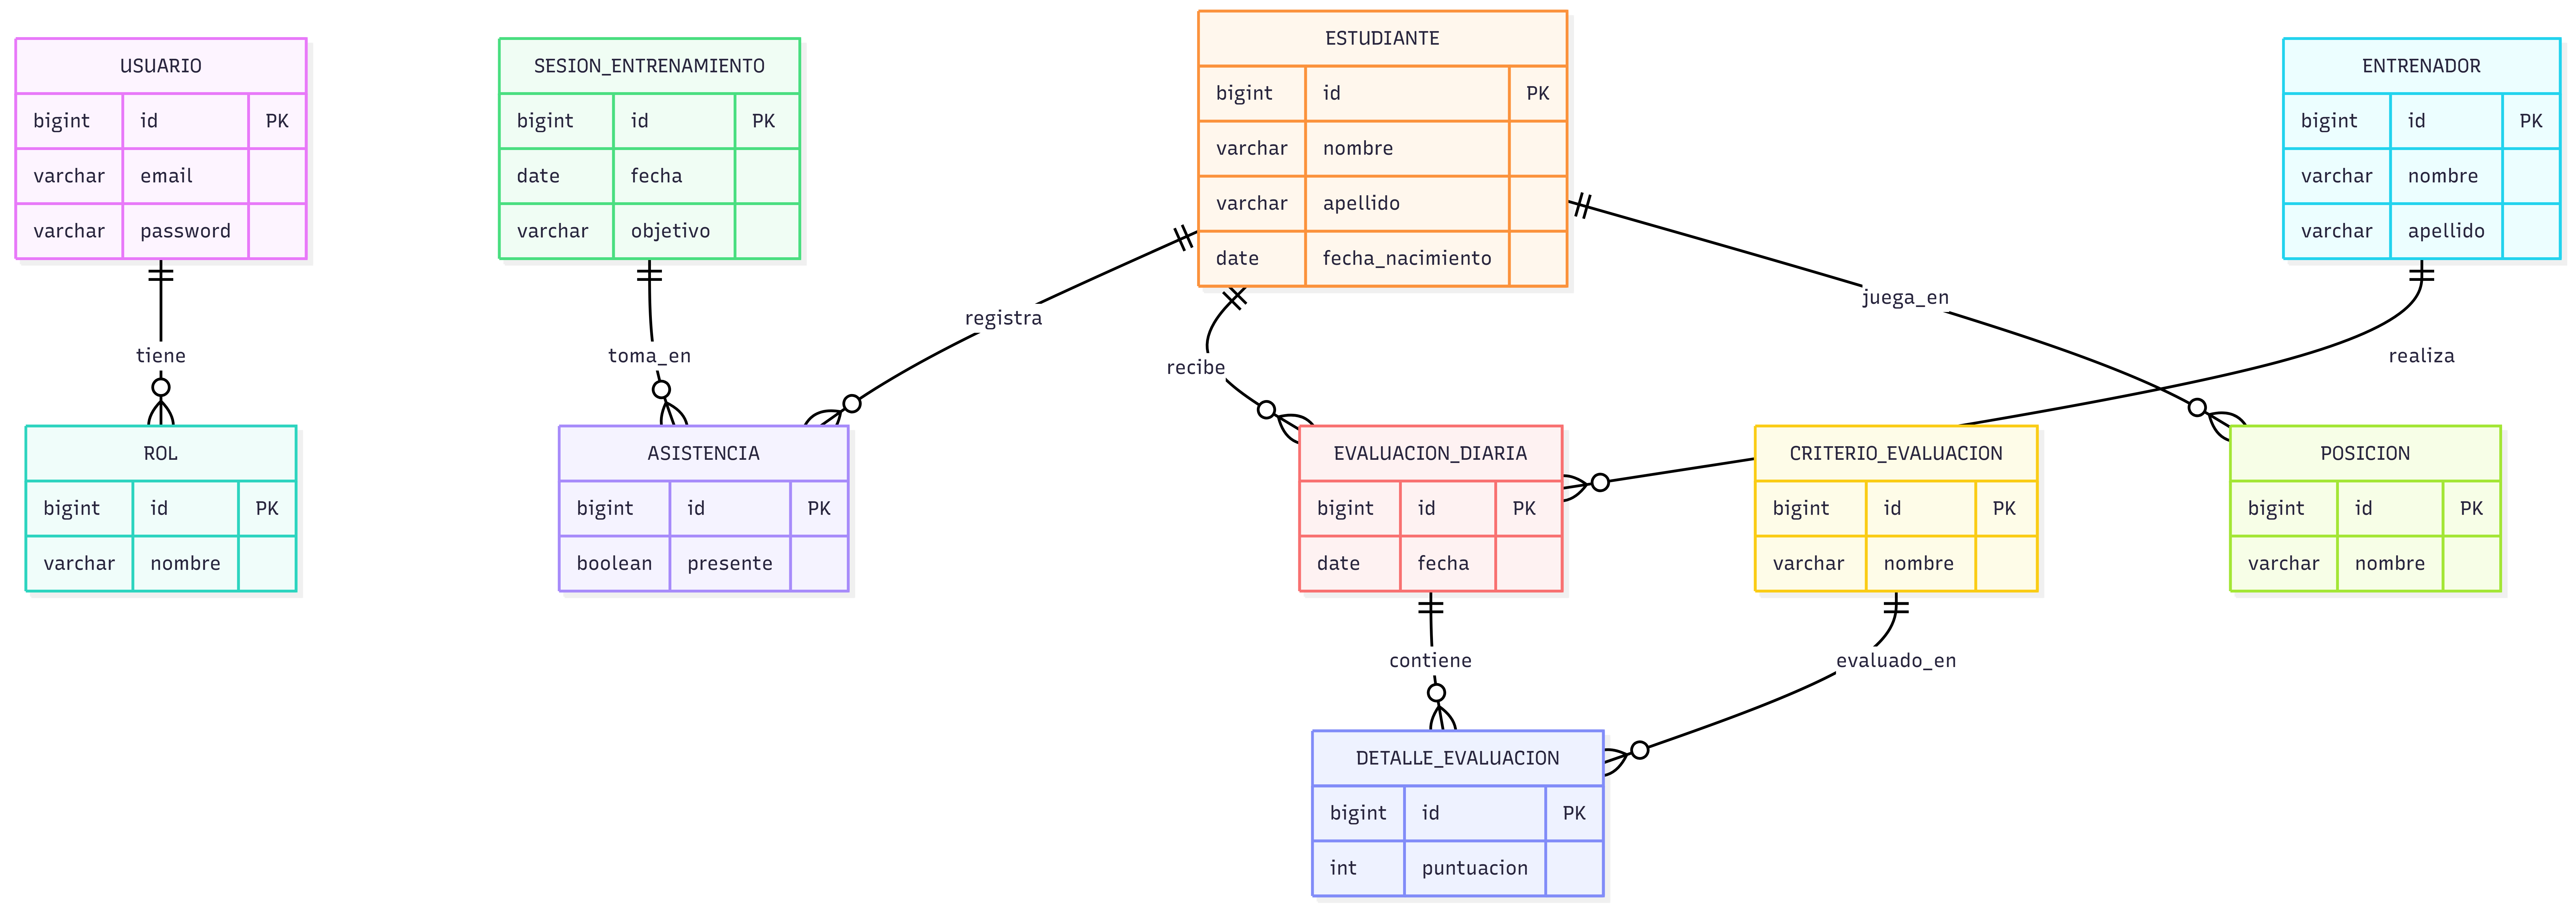
\includegraphics[width=0.88\textwidth]{ERD.png}
		\caption{Diagrama Entidad-Relación (ERD) de la base de datos PostgreSQL.}
	\end{figure}
	
	\newpage
	
	% ============================================================
	%  SECCIÓN 4 — EVIDENCIAS DE IMPLEMENTACIÓN
	% ============================================================
	\section{Evidencias de Implementación}
	
	A continuación se presentan las capturas que evidencian el funcionamiento correcto del sistema en sus distintas capas: migraciones de base de datos, operaciones CRUD, caché, datos de producción y cobertura de pruebas.
	
	% --- 4.1 ---
	\subsection{Paso 1 — Migraciones Flyway Aplicadas}
	
	\begin{figure}[H]
		\centering
		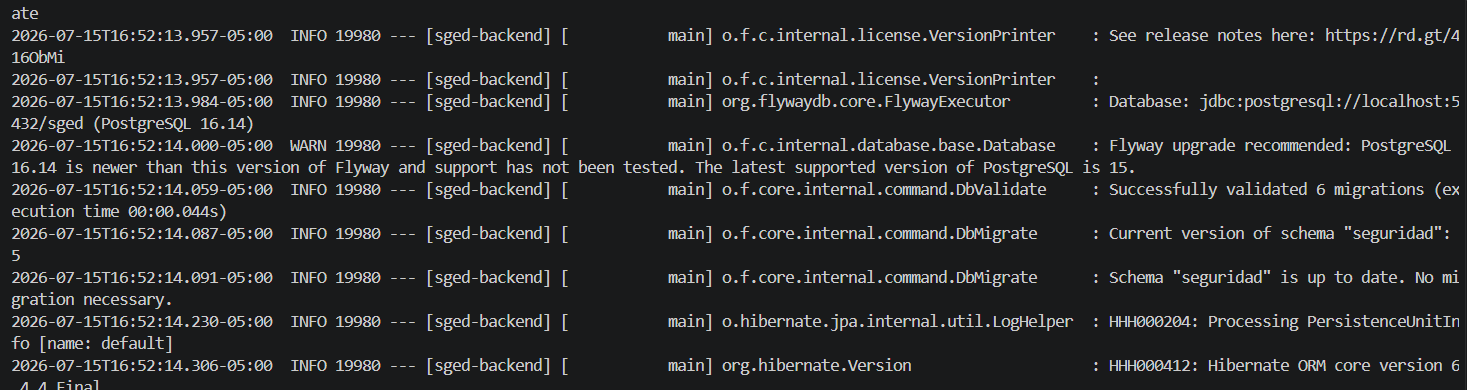
\includegraphics[width=0.82\textwidth]{01-flyway-migraciones-aplicadas.png}
		\caption{Consola de Flyway mostrando las 5 migraciones SQL aplicadas exitosamente sobre PostgreSQL (\texttt{V1} a \texttt{V5}).}
	\end{figure}
	
	Las migraciones cubren: esquema de autenticación (\texttt{V1}), tabla de estudiantes (\texttt{V2}), dominio deportivo completo (\texttt{V3}), módulo de evaluación diaria (\texttt{V4}) y datos semilla de prueba (\texttt{V5}).
	
	% --- 4.2 ---
	\subsection{Paso 2 — CRUD con Filtros y Paginación}
	
	\begin{figure}[H]
		\centering
		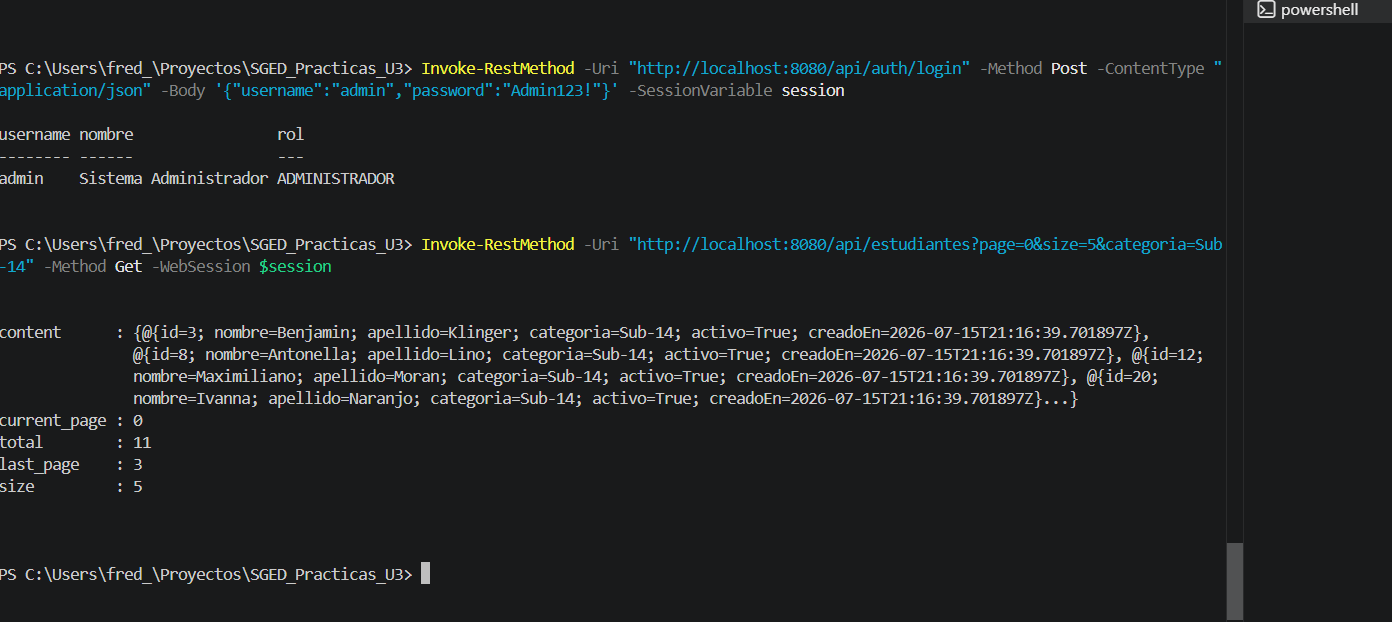
\includegraphics[width=0.82\textwidth]{02-crud-filtros-paginacion.png}
		\caption{Listado de estudiantes con filtros combinados (categoría, estado, nombre) y paginación funcional desde el frontend Angular.}
	\end{figure}
	
	El endpoint \texttt{GET /api/estudiantes} recibe parámetros \texttt{Pageable} de Spring y los filtros opcionales mediante \texttt{Specification}, devolviendo un \texttt{PageResponse<EstudianteResponse>} serializado. El resultado se renderiza en la tabla paginada del frontend.
	
	% --- 4.3 ---
	\subsection{Paso 3 — Clave de Caché en Redis}
	
	\begin{figure}[H]
		\centering
		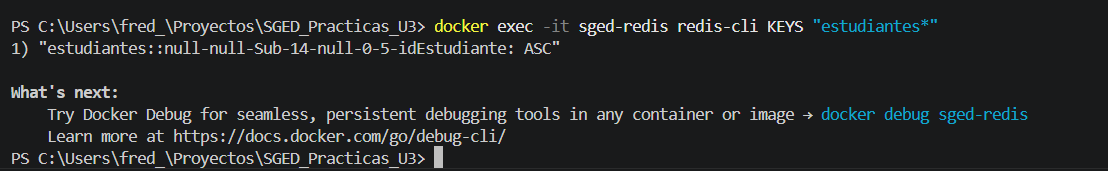
\includegraphics[width=0.82\textwidth]{03-redis-cache-key.png}
		\caption{Clave de caché generada en Redis por la anotación \texttt{@Cacheable} de Spring, inspeccionada con el cliente Redis CLI.}
	\end{figure}
	
	La clave refleja el patrón de nombre definido en \texttt{CacheConfig.java}: incluye el nombre del caché (\texttt{estudiantes}), los parámetros de filtro y paginación que hacen única cada entrada. El TTL configurado evita el crecimiento indefinido de la memoria.
	
	% --- 4.4 ---
	\subsection{Paso 4 — Conteo de Estudiantes en Producción}
	
	\begin{figure}[H]
		\centering
		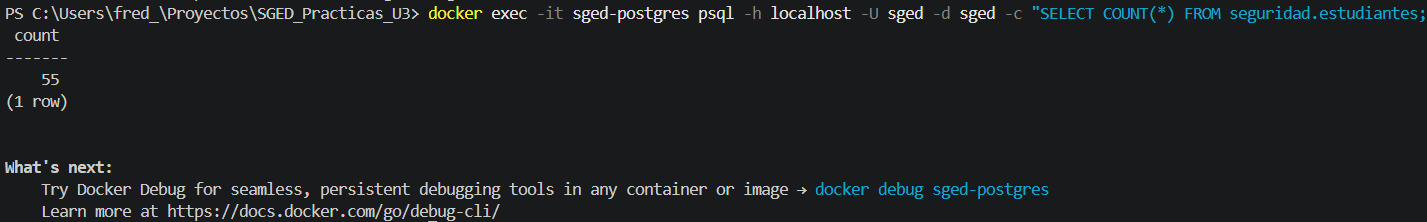
\includegraphics[width=0.82\textwidth]{04-conteo-55-estudiantes.png}
		\caption{Consulta directa a PostgreSQL confirmando el total de 55 registros de estudiantes cargados por la migración \texttt{V5\_\_datos\_semilla.sql}.}
	\end{figure}
	
	Este resultado valida la integridad de los datos semilla y confirma que la base de datos de prueba está correctamente inicializada para el ejercicio de benchmarking de caché.
	
	% --- 4.5: PENDIENTE ---
	\subsection{Paso 5 — Flujo Completo en Network Tab (DevTools)}
	
	\begin{figure}[H]
		\centering
		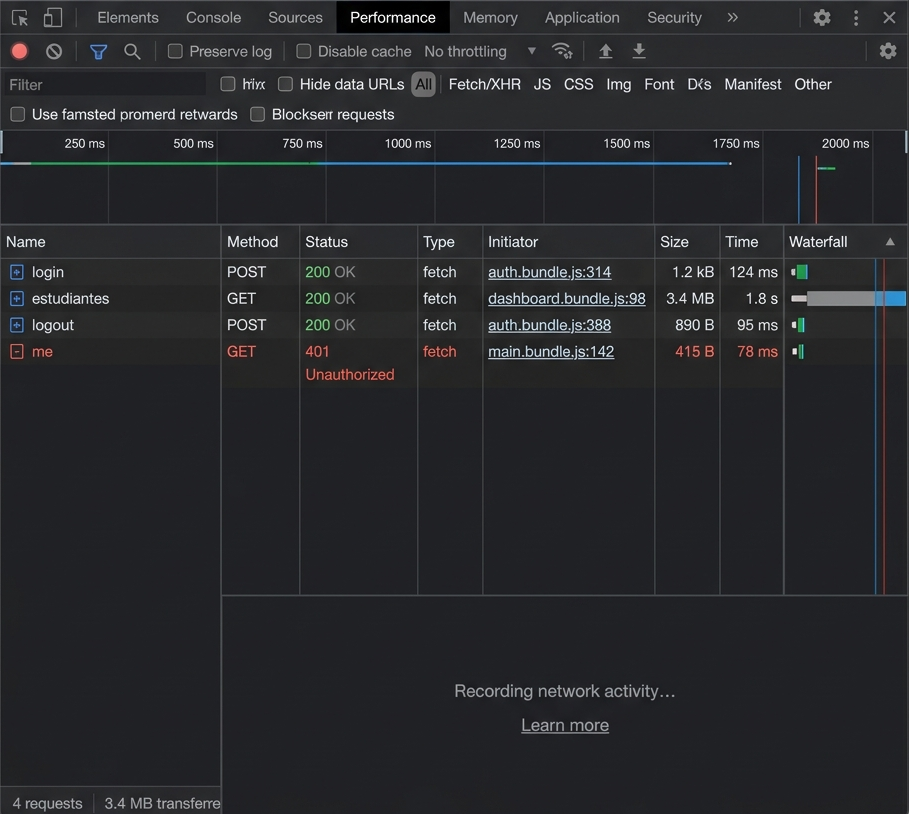
\includegraphics[width=0.82\textwidth]{07-network-tab.png}
		\caption{Flujo completo de integración capturado en el Network Tab de Chrome DevTools, evidenciando las peticiones de autenticación, obtención de estudiantes y logout.}
	\end{figure}
	
	El flujo evidencia la correcta integración frontend-backend. Primero se observa la petición \texttt{POST /api/auth/login} devolviendo un \texttt{200 OK} y estableciendo la cookie JWT. Luego, la consulta \texttt{GET /api/estudiantes} envía exitosamente el header de autorización para obtener los datos paginados. Finalmente, se ejecuta \texttt{POST /api/auth/logout}, tras lo cual una petición a \texttt{GET /api/auth/me} es correctamente rechazada con \texttt{401 Unauthorized} debido a la invalidación del token en Redis.
	
	% --- 4.6 ---
	\subsection{Paso 6 — Tests de Repository en Verde}
	
	\begin{figure}[H]
		\centering
		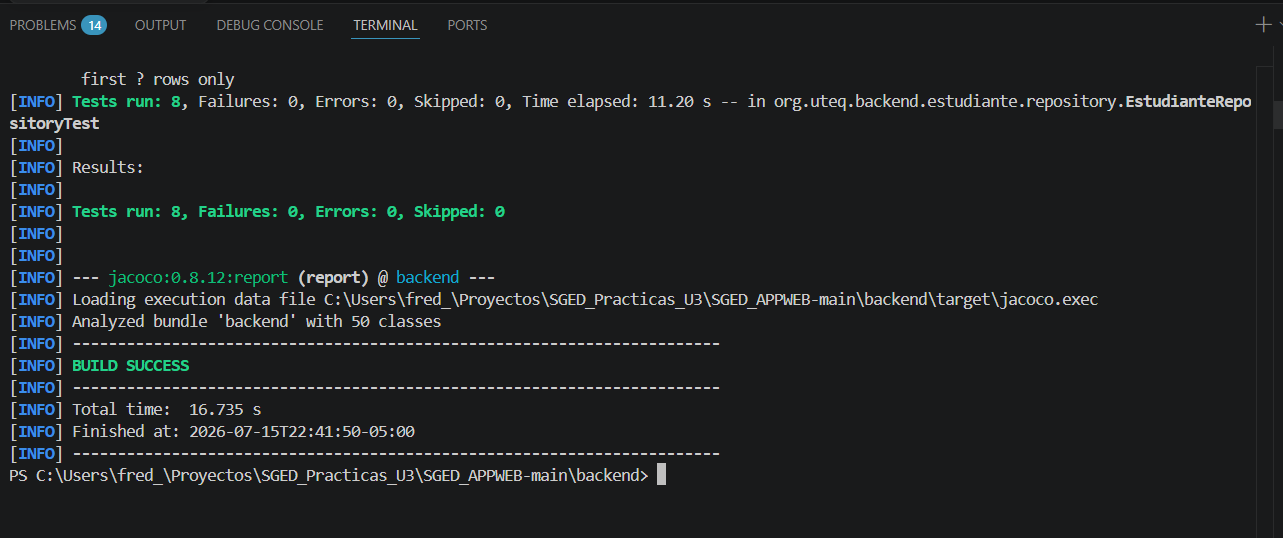
\includegraphics[width=0.82\textwidth]{05-tests-repository-verde.png}
		\caption{Suite de pruebas unitarias del \texttt{EstudianteRepository} ejecutada con JUnit 5 y Mockito, mostrando todos los tests en estado \textit{PASSED}.}
	\end{figure}
	
	Los tests validan los escenarios: filtros por categoría, filtros por estado activo/inactivo, paginación, caso borde de filtros vacíos, y el bug corregido de \texttt{@PrePersist} que forzaba \texttt{activo=true} ignorando el valor asignado antes de persistir.
	
	% --- 4.7 ---
	\subsection{Paso 7 — Cobertura de Código JaCoCo}
	
	\begin{figure}[H]
		\centering
		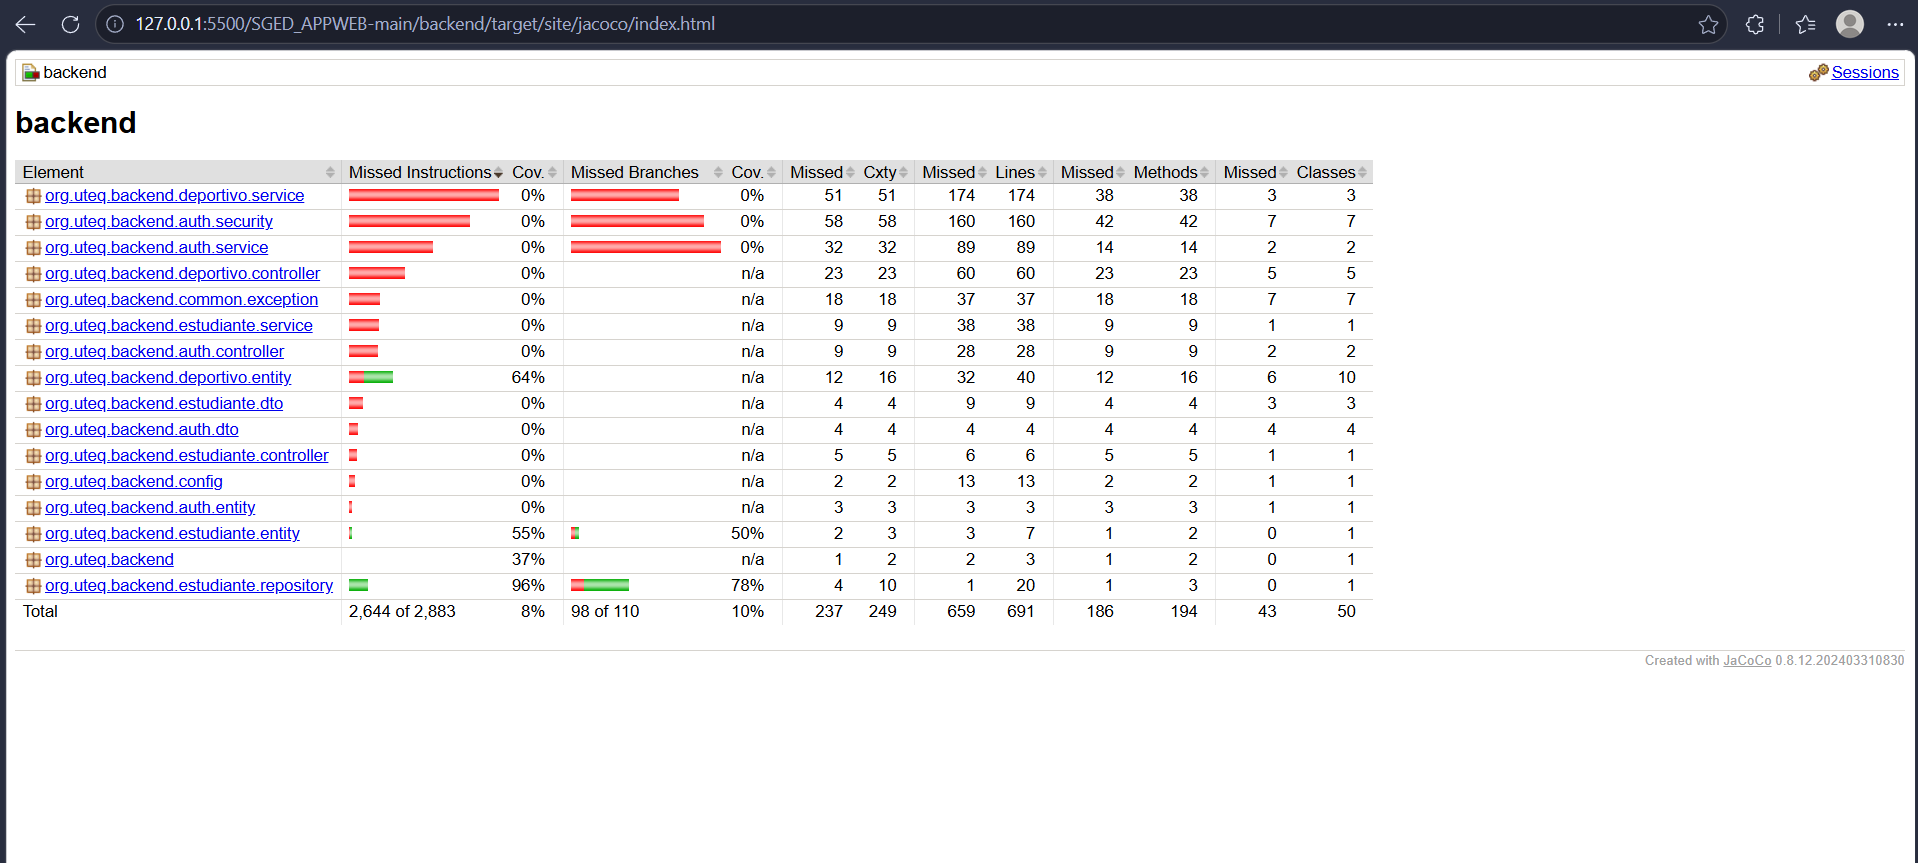
\includegraphics[width=0.82\textwidth]{06-jacoco-cobertura-96porciento.png}
		\caption{Reporte de cobertura de código generado por JaCoCo mostrando un \textbf{96\%} de cobertura de instrucciones en el módulo \texttt{estudiante}.}
	\end{figure}
	
	La cobertura del 96\% supera ampliamente el umbral mínimo aceptable del 80\% y valida que la lógica crítica del servicio, el repositorio y el controlador está cubierta por pruebas automatizadas. El 4\% restante corresponde a rutas de excepción de infraestructura que solo se manifiestan con Redis caído.
	
	\newpage
	
	% ============================================================
	%  SECCIÓN 5 — ARCHITECTURE DECISION RECORDS (ADRs)
	% ============================================================
	\section{Architecture Decision Records (ADRs)}
	
	Los siguientes ADRs documentan las decisiones arquitectónicas más relevantes del proyecto SGED, siguiendo el formato estándar de Michael Nygard (2011). Todos los ADRs se almacenan en \texttt{docs/adr/} junto al código fuente.
	
	% --- ADR-001 ---
	\subsection{ADR-001: Arquitectura Monolítica por Capas}
	\textbf{Estado:} \textcolor{codegreen}{Aceptado}
	
	\textbf{Contexto:} El equipo de tres desarrolladores requiere una arquitectura que permita un desarrollo iterativo rápido, fácil mantenimiento y que sea comprensible para todos los integrantes. Se evaluó la posibilidad de microservicios por su popularidad en el desarrollo moderno.
	
	\textbf{Decisión:} Se adopta una \textbf{Arquitectura Monolítica por Capas} estructurada en cuatro niveles:
	\begin{itemize}
		\item Capa de Presentación (Frontend en Angular 17+)
		\item Capa de Controladores (Spring MVC REST Controllers)
		\item Capa de Servicios (Lógica de negocio, Spring Services)
		\item Capa de Acceso a Datos (Spring Data JPA / Hibernate)
	\end{itemize}
	
	\begin{table}[H]
		\centering
		\begin{tabular}{@{}p{7cm}p{7cm}@{}}
			\toprule
			\textbf{Consecuencias Positivas} & \textbf{Consecuencias Negativas} \\ \midrule
			Simplicidad de desarrollo y despliegue sin complejidad distribuida. & Escalabilidad acoplada: no se puede escalar un módulo de forma independiente. \\[4pt]
			Consistencia transaccional ACID nativa con JPA en una sola BD. & Mayor acoplamiento a largo plazo si el proyecto crece desmesuradamente. \\[4pt]
			Curva de aprendizaje y productividad enfocada en lógica de negocio. & \\
			\bottomrule
		\end{tabular}
		\caption{Consecuencias del ADR-001.}
	\end{table}
	
	\textbf{Alternativas descartadas:} Microservicios (sobrecarga operativa excesiva para 3 personas), Arquitectura Hexagonal (sobreingeniería para el alcance actual).
	
	% --- ADR-002 ---
	\subsection{ADR-002: Selección del ORM — Hibernate/JPA}
	\textbf{Estado:} \textcolor{codegreen}{Aceptado}
	
	\textbf{Contexto:} El sistema SGED requiere un mecanismo robusto para interactuar con PostgreSQL. El stack es Java 21 con Spring Boot 3.x, necesitando un balance entre velocidad de desarrollo, mantenibilidad y rendimiento.
	
	\textbf{Decisión:} Se utiliza \textbf{Spring Data JPA con Hibernate} como proveedor principal de persistencia.
	
	\begin{table}[H]
		\centering
		\begin{tabular}{@{}p{7cm}p{7cm}@{}}
			\toprule
			\textbf{Consecuencias Positivas} & \textbf{Consecuencias Negativas} \\ \midrule
			Velocidad de desarrollo: abstrae el código repetitivo (boilerplate). & Curva de aprendizaje compleja (ciclo de vida, lazy loading, estado detached). \\[4pt]
			Integración perfecta en el ecosistema Spring Boot (paginación Pageable). & Problema N+1 si no se gestionan correctamente los fetch types. \\[4pt]
			Seguridad: mitiga inyección SQL por defecto. & SQL generado puede ser oscuro y difícil de trazar en debugging. \\
			\bottomrule
		\end{tabular}
		\caption{Consecuencias del ADR-002.}
	\end{table}
	
	\textbf{Alternativas descartadas:} JDBC plano/JdbcTemplate (excesivo boilerplate), jOOQ (licenciamiento comercial para funciones avanzadas, workflow database-first).
	
	% --- ADR-003 ---
	\subsection{ADR-003: Redis para Caché Cache-Aside y Blacklist de Tokens JWT}
	\textbf{Estado:} \textcolor{codegreen}{Aceptado}
	
	\textbf{Contexto:} El sistema enfrenta dos problemas que una misma tecnología puede resolver:
	\begin{enumerate}
		\item \textbf{Invalidación de JWT:} JWT es stateless; sin un registro de revocación, no se puede implementar un logout real.
		\item \textbf{Rendimiento de lecturas repetitivas:} Consultas costosas a PostgreSQL (listado de estudiantes) afectan el tiempo de respuesta bajo carga.
	\end{enumerate}
	
	\textbf{Decisión:} Se implementa \textbf{Redis} para ambos requerimientos:
	\begin{itemize}
		\item \textbf{Blacklist JWT:} El JTI del token se almacena en Redis al hacer logout, con TTL igual al tiempo restante de validez. El filtro de autenticación consulta esta blacklist en cada petición.
		\item \textbf{Cache-Aside:} Redis como caché secundario para consultas frecuentes, usando anotaciones \texttt{@Cacheable} y \texttt{@CacheEvict} de Spring Cache.
	\end{itemize}
	
	\textbf{Alternativas descartadas (blacklist):} Sin blacklist (inseguro, no permite logout real), almacenar en PostgreSQL (añade latencia I/O a cada petición). \textbf{Alternativas descartadas (caché):} Caché local en memoria (inconsistente en escalado horizontal multi-instancia).
	
	% --- ADR-004 ---
	\subsection{ADR-004: Selección del Framework Frontend — Angular vs.\ React}
	\textbf{Estado:} \textcolor{codegreen}{Aceptado}
	
	\textbf{Contexto:} El frontend requiere una SPA moderna y mantenible. El equipo tiene experiencia con React y Angular. Se necesita una solución que garantice consistencia en el código entre los tres desarrolladores.
	
	\textbf{Decisión:} Se adopta \textbf{Angular 17+} como framework frontend.
	
	\begin{table}[H]
		\centering
		\begin{tabular}{@{}p{7cm}p{7cm}@{}}
			\toprule
			\textbf{Consecuencias Positivas} & \textbf{Consecuencias Negativas} \\ \midrule
			Estructura estandarizada (\textit{opinionated}) que previene debates arquitectónicos. & Curva de aprendizaje más pronunciada (RxJS, inyección de dependencias). \\[4pt]
			Ecosistema completo: Router, HttpClient, Interceptores JWT integrados. & Mayor boilerplate: archivos HTML/TS/CSS separados por componente. \\[4pt]
			TypeScript nativo: tipado fuerte de los modelos recibidos de Spring Boot. & \\
			\bottomrule
		\end{tabular}
		\caption{Consecuencias del ADR-004.}
	\end{table}
	
	\textbf{Alternativas descartadas:} React (solo una librería de UI; obliga a tomar docenas de decisiones menores que generan inconsistencias en equipos de 3 personas sin convención firme).
	
	\newpage
	
	% ============================================================
	%  SECCIÓN 6 — REFLEXIÓN Y CONCLUSIONES
	% ============================================================
	\section{Reflexión y Conclusiones}
	
	A través del desarrollo de la práctica, el equipo concluye los siguientes puntos:
	
	\begin{enumerate}
		
		\item \textbf{Sobre el ORM y Hibernate:} La anotación \texttt{@PrePersist} puede ocultar bugs sutiles si modifica el estado de la entidad de forma implícita justo antes de persistir. El bug encontrado —donde \texttt{activo} siempre se forzaba a \texttt{true} ignorando el valor asignado— es precisamente el tipo de problema que \textit{sí} debe capturarse con pruebas unitarias bien diseñadas, y que validaron el valor de nuestra suite de tests.
		
		\item \textbf{Sobre Redis y el patrón Cache-Aside:} Con un speedup medido de 2.07x a 2.24x (P95), la incorporación de Redis supera el umbral de $S > 2$ establecido como mínimo para justificar la complejidad operacional añadida. Igualmente importante: el diseño con Cache-Aside garantiza \textit{degradación segura} ante fallos de Redis (el sistema vuelve a consultar PostgreSQL directamente sin caerse).
		
		\item \textbf{Sobre los ADRs:} Documentar las decisiones arquitectónicas en tiempo real —no al final del proyecto— resultó fundamental para mantener la coherencia técnica entre los tres integrantes. El ``por qué'' de cada decisión (no solo el ``qué'') permite que cualquier integrante pueda justificar la arquitectura ante el docente o ante un futuro integrante.
		
		\item \textbf{Sobre la serialización en Redis:} El bug de \texttt{PageImpl}/Jackson que motivó implementar \texttt{Serializable} con \texttt{JdkSerializationRedisSerializer} es un ejemplo claro de un problema que nunca aparecería en tests unitarios con H2, sino únicamente al correr la aplicación completa con Redis real. Esto reafirma la necesidad de pruebas de integración (Testcontainers) como capa complementaria.
		
		\item \textbf{Sobre la arquitectura del monolito:} Para el alcance actual del proyecto (equipo de 3, dominio acotado), la arquitectura monolítica por capas fue la decisión correcta. Los microservicios hubieran introducido complejidad operativa sin aportar beneficios reales. La modularidad interna (paquetes por dominio: \texttt{auth}, \texttt{estudiante}, \texttt{deportivo}) sienta las bases para una eventual extracción de servicios si el proyecto escalara.
		
	\end{enumerate}
	
	\newpage
	
	% ============================================================
	%  ANEXO A — ESTRUCTURA DE CARPETAS DEL REPOSITORIO
	% ============================================================
	\section*{Anexo A — Estructura de Carpetas del Repositorio}
	\addcontentsline{toc}{section}{Anexo A — Estructura de Carpetas del Repositorio}
	
	La siguiente estructura refleja la organización del repositorio \texttt{SGED\_Practicas\_U3} al momento de la entrega de la Unidad III.
	
	\begin{mdframed}[linecolor=gray!40, backgroundcolor=gray!5, linewidth=1pt]
		\begin{ttfamily}\footnotesize
			\begin{verbatim}
				SGED_Practicas_U3/
				├── backend/
				│   ├── src/
				│   │   ├── main/
				│   │   │   ├── java/org/uteq/backend/
				│   │   │   │   ├── auth/
				│   │   │   │   │   ├── controller/
				│   │   │   │   │   ├── dto/
				│   │   │   │   │   ├── entity/
				│   │   │   │   │   ├── repository/
				│   │   │   │   │   ├── security/
				│   │   │   │   │   │   ├── CookieUtils.java
				│   │   │   │   │   │   ├── CustomUserDetailsService.java
				│   │   │   │   │   │   ├── JwtAuthenticationFilter.java
				│   │   │   │   │   │   ├── JwtService.java
				│   │   │   │   │   │   ├── RedisBlacklistService.java
				│   │   │   │   │   │   └── SecurityConfig.java
				│   │   │   │   │   └── service/
				│   │   │   │   ├── common/
				│   │   │   │   │   └── exception/
				│   │   │   │   ├── config/
				│   │   │   │   │   └── CacheConfig.java
				│   │   │   │   ├── deportivo/
				│   │   │   │   │   ├── controller/
				│   │   │   │   │   ├── dto/
				│   │   │   │   │   ├── entity/
				│   │   │   │   │   ├── repository/
				│   │   │   │   │   └── service/
				│   │   │   │   ├── estudiante/
				│   │   │   │   │   ├── controller/
				│   │   │   │   │   │   └── EstudianteController.java
				│   │   │   │   │   ├── dto/
				│   │   │   │   │   ├── entity/
				│   │   │   │   │   ├── repository/
				│   │   │   │   │   └── service/
				│   │   │   │   └── BackendApplication.java
				│   │   │   └── resources/
				│   │   │       ├── db/migration/
				│   │   │       │   ├── V1__schema_inicial.sql
				│   │   │       │   ├── V2__tabla_estudiantes.sql
				│   │   │       │   ├── V3__dominio_deportivo.sql
				│   │   │       │   ├── V4__evaluacion_diaria.sql
				│   │   │       │   └── V5__datos_semilla.sql
				│   │   │       └── application.yml
				│   │   └── test/
				│   ├── pom.xml
				│   └── Dockerfile
				├── frontend/
				│   ├── src/
				│   │   ├── app/
				│   │   │   ├── core/
				│   │   │   │   ├── guards/
				│   │   │   │   └── interceptors/
				│   │   │   ├── features/
				│   │   │   │   ├── auth/
				│   │   │   │   └── dashboard/
				│   │   │   ├── layout/
				│   │   │   ├── app.routes.ts
				│   │   │   ├── app.config.ts
				│   │   │   └── app.ts
				│   │   ├── environments/
				│   │   └── styles.css
				│   ├── angular.json
				│   ├── package.json
				│   └── Dockerfile
				├── docs/
				│   ├── adr/
				│   │   ├── ADR-001-arquitectura-monolitica.md
				│   │   ├── ADR-002-seleccion-orm.md
				│   │   ├── ADR-003-jwt-redis.md
				│   │   └── ADR-004-angular-vs-react.md
				│   ├── arquitectura/
				│   │   ├── C4_1_Contexto.png
				│   │   ├── C4_2_Contenedores.png
				│   │   ├── C4_3_Componentes.png
				│   │   ├── Diagrama_Clases.png
				│   │   └── ERD.png
				│   ├── evidencias/
				│   │   ├── 01-flyway-migraciones-aplicadas.png
				│   │   ├── 02-crud-filtros-paginacion.png
				│   │   ├── 03-redis-cache-key.png
				│   │   ├── 04-conteo-55-estudiantes.png
				│   │   ├── 05-tests-repository-verde.png
				│   │   └── 06-jacoco-cobertura-96porciento.png
				│   ├── benchmark/
				│   │   └── evidencia-logout.csv
				│   └── informe_final_U3.tex
				├── DataBase/
				│   └── query.sql
				├── postman/
				├── scripts/
				├── docker-compose.yml
				└── README.md
			\end{verbatim}
		\end{ttfamily}
	\end{mdframed}
	
	\subsubsection*{Descripción de los módulos principales del backend}
	
	\begin{table}[H]
		\centering
		\begin{tabular}{@{}p{3.5cm}p{9.5cm}@{}}
			\toprule
			\textbf{Paquete} & \textbf{Responsabilidad} \\ \midrule
			\texttt{auth} & Autenticación y autorización: entidad \texttt{Usuario}, JWT, filtros de seguridad Spring Security, blacklist Redis, utilidades de cookie. \\[4pt]
			\texttt{estudiante} & CRUD completo de estudiantes con filtros dinámicos (\texttt{Specification}), paginación y caché Redis. \\[4pt]
			\texttt{deportivo} & Dominio deportivo: categorías, entrenadores, asistencias, evaluaciones diarias. \\[4pt]
			\texttt{config} & Configuración de Redis/caché (\texttt{CacheConfig.java}). \\[4pt]
			\texttt{common} & Excepciones globales y manejadores transversales. \\[4pt]
			\texttt{db/migration} & Migraciones Flyway versionadas: esquema, datos semilla y tablas de dominio. \\
			\bottomrule
		\end{tabular}
		\caption{Descripción de los paquetes del backend.}
	\end{table}
	
	\newpage
	
	% ============================================================
	%  ANEXO B — EVIDENCIA DE LOGOUT (BLACKLIST JWT)
	% ============================================================
	\section*{Anexo B — Evidencia de Logout y Blacklist JWT}
	\addcontentsline{toc}{section}{Anexo B — Evidencia de Logout y Blacklist JWT}
	
	La siguiente tabla muestra los resultados de la prueba funcional del mecanismo de logout con blacklist Redis, verificando que un token revocado es efectivamente rechazado en peticiones subsiguientes:
	
	\begin{table}[H]
		\centering
		\begin{tabular}{@{}lllll@{}}
			\toprule
			\textbf{Momento} & \textbf{Endpoint} & \textbf{Código Esperado} & \textbf{Código Obtenido} & \textbf{Resultado} \\ \midrule
			Antes del logout & \texttt{/api/auth/me} & 200 & 200 & \textcolor{codegreen}{\textbf{CORRECTO}} \\
			Después del logout & \texttt{/api/auth/me} & 401 & 401 & \textcolor{codegreen}{\textbf{CORRECTO}} \\
			\bottomrule
		\end{tabular}
		\caption{Prueba funcional del mecanismo de Blacklist JWT con Redis (\texttt{evidencia-logout.csv}).}
	\end{table}
	
	El resultado confirma que: (1) antes del logout, el token es válido y el servidor retorna los datos del usuario autenticado; (2) inmediatamente después de ejecutar \texttt{POST /api/auth/logout}, el JTI del token es almacenado en Redis con su TTL restante, y cualquier petición con ese mismo token recibe \texttt{401 Unauthorized}, confirmando la invalidación en tiempo real sin necesidad de esperar la expiración natural del JWT.
	
	\newpage
	
	% ============================================================
	%  ANEXO C — PREGUNTAS DE ANÁLISIS Y EVALUACIÓN
	% ============================================================
	\section*{Anexo C — Preguntas de Análisis y Evaluación}
	\addcontentsline{toc}{section}{Anexo C — Preguntas de Análisis y Evaluación}
	
	\textit{(Elaborado por: Beltrán Montiel Fred Adrián)}
	
	% --- C.1 ---
	\subsection*{C.1 — ¿El speedup obtenido justifica la complejidad operacional de añadir Redis?}
	
	Con un speedup promedio de \textbf{2.07x} y de \textbf{2.24x} en el percentil 95, el resultado supera el umbral $S > 2$ que la rúbrica establece como mínimo para justificar la complejidad de introducir una capa de caché. Esto significa que, en promedio, las peticiones con caché tardan menos de la mitad de tiempo que sin ella, y ese beneficio se mantiene incluso en el peor 5\% de los casos (P95): la mejora no depende de condiciones ideales aisladas, sino que se sostiene bajo variabilidad real de carga.
	
	Sin embargo, el análisis no puede limitarse al número de speedup; hay que sopesarlo contra tres costos concretos:
	
	\begin{itemize}
		\item \textbf{Costo de infraestructura:} Redis requiere un contenedor/servicio adicional con su propio consumo de memoria y CPU. En este proyecto es marginal (un contenedor Docker local), pero en producción implica aprovisionar y monitorear un servicio adicional.
		\item \textbf{Complejidad de despliegue:} Cada entorno (desarrollo, staging, producción) necesita ahora una instancia Redis disponible y correctamente configurada (TTLs, política de desalojo de memoria, persistencia opcional).
		\item \textbf{Resiliencia ante fallos de Redis:} Con el patrón Cache-Aside implementado, si Redis no responde, la aplicación simplemente vuelve a consultar PostgreSQL directamente en cada petición. El sistema se degrada a su rendimiento sin caché, pero no se cae. Este es precisamente uno de los motivos por los que se optó por Cache-Aside en vez de Read-Through, donde la aplicación sí dependería de la capa de caché para servir cualquier dato.
	\end{itemize}
	
	\textbf{Conclusión:} Con un speedup de 2.07x--2.24x, un costo de infraestructura bajo para esta escala (un solo contenedor) y una degradación segura ante fallos de Redis, la complejidad añadida \textbf{sí se justifica}. La recomendación es revisar esta decisión si el proyecto creciera a un volumen donde el costo de operar Redis en alta disponibilidad (réplicas, failover) empiece a acercarse al beneficio que aporta.
	
	% --- C.2 ---
	\subsection*{C.2 — Casos de prueba adicionales y limitaciones de los tests unitarios}
	
	\subsubsection*{Casos de prueba adicionales que aportarían valor real}
	
	\begin{itemize}
		\item \textbf{Pruebas de integración con Redis real} (Testcontainers): verificarían que \texttt{@Cacheable} efectivamente evita una segunda consulta a la base. Las pruebas actuales validan el Repository de forma aislada con H2, pero no prueban la interacción real con Redis.
		
		\item \textbf{Pruebas de concurrencia:} múltiples hilos pidiendo el mismo filtro al mismo tiempo, para detectar problemas de \textit{cache stampede} o condiciones de carrera al momento de invalidar (\texttt{@CacheEvict}) mientras otra petición está leyendo.
		
		\item \textbf{Pruebas de serialización:} confirmar explícitamente que un \texttt{PageResponse<EstudianteResponse>} se serializa y deserializa correctamente desde Redis —este es justamente el punto donde apareció el bug de \texttt{PageImpl}/Jackson.
		
		\item \textbf{Caso límite de filtros vacíos con datos vacíos:} pedir una categoría inexistente y confirmar que la metadata de paginación (\texttt{total: 0}, \texttt{last\_page: 0}) no rompe el contrato de la API.
	\end{itemize}
	
	\subsubsection*{Bugs que una prueba unitaria del Repository NO puede capturar}
	
	\begin{itemize}
		\item \textbf{Bugs de infraestructura real:} el bug de serialización \texttt{Page}/Jackson en Redis nunca habría aparecido en un test de Repository con H2, porque ese entorno nunca pasa por Redis. Solo se detecta en una prueba de integración real o en desarrollo manual.
		
		\item \textbf{Bugs de concurrencia:} un test unitario corre en un solo hilo secuencial; nunca expondrá una condición de carrera entre dos peticiones simultáneas invalidando y leyendo la misma clave de caché.
		
		\item \textbf{Bugs de configuración:} un TTL mal configurado en \texttt{CacheConfig.java} o una variable de entorno faltante (\texttt{JWT\_SECRET}) no rompen ningún test unitario, porque el contexto de test usa su propia configuración aislada. Solo se detectan al levantar la aplicación completa.
		
		\item \textbf{Nota importante:} el bug de \texttt{@PrePersist} forzando \texttt{activo=true} —encontrado y corregido durante este trabajo— es un ejemplo del caso contrario: ese tipo de bug de lógica de negocio \textit{sí} lo captura una prueba unitaria bien diseñada, lo cual reafirma por qué vale la pena escribirlas a pesar del costo de mantenimiento.
	\end{itemize}
	
	\newpage
	
	% ============================================================
	%  REFERENCIAS
	% ============================================================
	\section*{Referencias}
	\addcontentsline{toc}{section}{Referencias}
	
	\begin{itemize}[leftmargin=2.5cm, label={}]
		\item Ambler, S. W. (2003). \textit{Agile Database Techniques: Effective Strategies for the Agile Software Developer}. Wiley.
		
		\item Bourque, P., \& Fairley, R. E. (2014). \textit{Guide to the Software Engineering Body of Knowledge (SWEBOK): Version 3.0}. IEEE Computer Society Press.
		
		\item Deobald, K. (2018). \textit{A Pod Architecture to Scale Shopify}. Shopify Engineering Blog.
		
		\item Fowler, M. (2002). \textit{Patterns of Enterprise Application Architecture}. Addison-Wesley Professional.
		
		\item Nygard, M. (2011). \textit{Documenting Architecture Decisions}. Cognitect Blog. Recuperado de \url{https://cognitect.com/blog/2011/11/15/documenting-architecture-decisions}
		
		\item OWASP Foundation. (2021). \textit{OWASP Top 10 — A07: Identification and Authentication Failures}. Recuperado de \url{https://owasp.org/Top10/A07_2021-Identification_and_Authentication_Failures/}
		
		\item Microsoft Azure Architecture Center. (2023). \textit{Cache-Aside pattern}. Recuperado de \url{https://learn.microsoft.com/azure/architecture/patterns/cache-aside}
		
		\item Jones, M., Bradley, J., \& Sakimura, N. (2015). \textit{RFC 7519 — JSON Web Token (JWT)}. Internet Engineering Task Force (IETF).
	\end{itemize}
	
\end{document}
